% LEAF 1015 版合稿入口。编译：tectonic main.tex，或 pdfLaTeX + BibTeX（Overleaf 默认）。
% 各章源文件位于 sections/ 下对应子目录，参考文献统一使用本目录 references.bib。
% 第三章有两个版本：本文件给出固定翼载具细节；main_generic.tex 先定义 \LEAFGenericVehicle，
% 得到不含载具细节的通用描述版本，其余各章两版相同。
\RequirePackage[T1]{fontenc}
\documentclass[journal,10pt]{IEEEtran}
\usepackage{amsmath,amssymb}
\usepackage{algorithm,algorithmic}
\usepackage{array,booktabs,multirow}
\usepackage{graphicx,xcolor}
\usepackage{tikz}
\usetikzlibrary{arrows.meta,positioning,fit,calc}
\usepackage{cite,url}
\usepackage[hidelinks]{hyperref}

\newtheorem{proposition}{Proposition}
\renewcommand{\algorithmiccomment}[1]{\hfill$\triangleright$~#1}
\hyphenation{multi-agent gene-ra-li-za-tion re-pre-sen-ta-tion}
\hypersetup{pdftitle={Looped Threat Context Reasoning for Scalable Multiagent Target Defense}}

\newif\ifvehicledetail
\ifdefined\LEAFGenericVehicle\vehicledetailfalse\else\vehicledetailtrue\fi

\begin{document}
\bstctlcite{leafBibliographyControl}
% =====================================================================
% 1015 版前置部分：标题、作者、摘要、Note to Practitioners、Index Terms
% 版式：IEEEtran journal（TASE）。在 main.tex 的 \begin{document} 之后直接
%   % =====================================================================
% 1015 版前置部分：标题、作者、摘要、Note to Practitioners、Index Terms
% 版式：IEEEtran journal（TASE）。在 main.tex 的 \begin{document} 之后直接
%   % =====================================================================
% 1015 版前置部分：标题、作者、摘要、Note to Practitioners、Index Terms
% 版式：IEEEtran journal（TASE）。在 main.tex 的 \begin{document} 之后直接
%   \input{sections/sec_1_2/front_matter}
% 本文件和 introduction.tex、related_work.tex 用到的文献都在同目录 references.bib。
% 摘要与引言中的数字来自 Open-SCORE/outputs/main/had/aggregates.json
% （comparison、design_comparison）和 Open-SCORE/outputs/main/summary.json
% （nomem_depth_analysis）。平台统一写作 SkyHAD 空中攻防环境，不点明动力学模型。
% =====================================================================

% 推荐标题。备选：
%   Looped Threat-Context Reasoning for Zero-Shot Scalable Multi-Target Defense
%   Train Small, Defend Large: Looped Threat Context Reasoning for Multiagent Target Defense
\title{Looped Threat Context Reasoning for\\ Scalable Multiagent Target Defense}

% 作者与首页脚注占位，投稿前替换。
\author{First~Author, Second~Author, and Third~Author%
\thanks{Manuscript received Month DD, 2026. This work was supported by ...}%
\thanks{The authors are with ... (e-mail: ...).}%
}

\markboth{IEEE Transactions on Automation Science and Engineering}%
{Looped Threat Context Reasoning for Scalable Multiagent Target Defense}

\maketitle

% 摘要单段，上限 200 词。叙述中的数字只保留训练与部署规模一处，优势用可核对的定性表述（不写 significantly）。
\begin{abstract}
Multiagent target defense requires defenders to protect several assets from attackers. Because team and asset counts are rarely known in advance, a policy should train once on small engagements and transfer to larger ones. Transfer is hard because an attacker's threat depends on the target it approaches and on the teammates already covering it. We call this relation the threat context. We propose Looped Entity Attention with Fused reading (LEAF), which builds this context by looping one weight-shared entity-attention operator. A query formed from the defender's current state reads every round, the reads are fused, and recurrent memory enters only after reading. Training samples the number of rounds, so the policy can act after any round. In the SkyHAD aerial defense environment, policies trained with at most 10 defenders and 3 targets transfer without retraining to 50 defenders or 12 targets. LEAF has the lowest target damage in every test configuration, and in every test group even its weakest training run beats the best run of each baseline. Ablations confirm the roles of context construction, multi-round refinement, and memory placement. With a single round of reasoning, LEAF keeps nearly all of its protection, whereas a fixed-depth model collapses.
\end{abstract}

% TASE 要求的 Note to Practitioners，用非专业语言写实际用途、潜力与局限，正文 200 词（要求 100--300 词）。
% 借用 abstract 环境排版，使其与摘要同样式，显示为 Note to Practitioners---。
{\renewcommand{\abstractname}{Note to Practitioners}%
\begin{abstract}
Teams of autonomous aircraft that guard airports, ports, or industrial sites must handle attacks whose size is unknown in advance. This work provides one control policy that is trained in small simulated engagements and then runs unchanged with several times more defenders, attackers, and protected sites. Every defender runs a copy of the same network on the positions, velocities, and status of the aircraft and sites it observes, and the network returns its next maneuver. Adding aircraft or sites needs no retraining, because all entities share the same parameters. The network first relates each attacker to the protected sites and nearby defenders, then interprets this picture from the defender's own situation, and only afterward uses its memory of earlier steps. Operators can also set how many reasoning rounds the network runs. A single round already keeps nearly all of the protection, so the controller can be matched to the onboard computer and the required decision rate without training a new model. The policy has so far been tested in simulation, where the defenders see every aircraft and site and the attackers follow a fixed rule. Field use calls for further tests with onboard sensors, communication delays, and attackers that adapt their tactics.
\end{abstract}}

\begin{IEEEkeywords}
Multiagent reinforcement learning, multi-target defense, scale generalization, entity attention, iterative reasoning, unmanned aerial vehicles.
\end{IEEEkeywords}

% 本文件和 introduction.tex、related_work.tex 用到的文献都在同目录 references.bib。
% 摘要与引言中的数字来自 Open-SCORE/outputs/main/had/aggregates.json
% （comparison、design_comparison）和 Open-SCORE/outputs/main/summary.json
% （nomem_depth_analysis）。平台统一写作 SkyHAD 空中攻防环境，不点明动力学模型。
% =====================================================================

% 推荐标题。备选：
%   Looped Threat-Context Reasoning for Zero-Shot Scalable Multi-Target Defense
%   Train Small, Defend Large: Looped Threat Context Reasoning for Multiagent Target Defense
\title{Looped Threat Context Reasoning for\\ Scalable Multiagent Target Defense}

% 作者与首页脚注占位，投稿前替换。
\author{First~Author, Second~Author, and Third~Author%
\thanks{Manuscript received Month DD, 2026. This work was supported by ...}%
\thanks{The authors are with ... (e-mail: ...).}%
}

\markboth{IEEE Transactions on Automation Science and Engineering}%
{Looped Threat Context Reasoning for Scalable Multiagent Target Defense}

\maketitle

% 摘要单段，上限 200 词。叙述中的数字只保留训练与部署规模一处，优势用可核对的定性表述（不写 significantly）。
\begin{abstract}
Multiagent target defense requires defenders to protect several assets from attackers. Because team and asset counts are rarely known in advance, a policy should train once on small engagements and transfer to larger ones. Transfer is hard because an attacker's threat depends on the target it approaches and on the teammates already covering it. We call this relation the threat context. We propose Looped Entity Attention with Fused reading (LEAF), which builds this context by looping one weight-shared entity-attention operator. A query formed from the defender's current state reads every round, the reads are fused, and recurrent memory enters only after reading. Training samples the number of rounds, so the policy can act after any round. In the SkyHAD aerial defense environment, policies trained with at most 10 defenders and 3 targets transfer without retraining to 50 defenders or 12 targets. LEAF has the lowest target damage in every test configuration, and in every test group even its weakest training run beats the best run of each baseline. Ablations confirm the roles of context construction, multi-round refinement, and memory placement. With a single round of reasoning, LEAF keeps nearly all of its protection, whereas a fixed-depth model collapses.
\end{abstract}

% TASE 要求的 Note to Practitioners，用非专业语言写实际用途、潜力与局限，正文 200 词（要求 100--300 词）。
% 借用 abstract 环境排版，使其与摘要同样式，显示为 Note to Practitioners---。
{\renewcommand{\abstractname}{Note to Practitioners}%
\begin{abstract}
Teams of autonomous aircraft that guard airports, ports, or industrial sites must handle attacks whose size is unknown in advance. This work provides one control policy that is trained in small simulated engagements and then runs unchanged with several times more defenders, attackers, and protected sites. Every defender runs a copy of the same network on the positions, velocities, and status of the aircraft and sites it observes, and the network returns its next maneuver. Adding aircraft or sites needs no retraining, because all entities share the same parameters. The network first relates each attacker to the protected sites and nearby defenders, then interprets this picture from the defender's own situation, and only afterward uses its memory of earlier steps. Operators can also set how many reasoning rounds the network runs. A single round already keeps nearly all of the protection, so the controller can be matched to the onboard computer and the required decision rate without training a new model. The policy has so far been tested in simulation, where the defenders see every aircraft and site and the attackers follow a fixed rule. Field use calls for further tests with onboard sensors, communication delays, and attackers that adapt their tactics.
\end{abstract}}

\begin{IEEEkeywords}
Multiagent reinforcement learning, multi-target defense, scale generalization, entity attention, iterative reasoning, unmanned aerial vehicles.
\end{IEEEkeywords}

% 本文件和 introduction.tex、related_work.tex 用到的文献都在同目录 references.bib。
% 摘要与引言中的数字来自 Open-SCORE/outputs/main/had/aggregates.json
% （comparison、design_comparison）和 Open-SCORE/outputs/main/summary.json
% （nomem_depth_analysis）。平台统一写作 SkyHAD 空中攻防环境，不点明动力学模型。
% =====================================================================

% 推荐标题。备选：
%   Looped Threat-Context Reasoning for Zero-Shot Scalable Multi-Target Defense
%   Train Small, Defend Large: Looped Threat Context Reasoning for Multiagent Target Defense
\title{Looped Threat Context Reasoning for\\ Scalable Multiagent Target Defense}

% 作者与首页脚注占位，投稿前替换。
\author{First~Author, Second~Author, and Third~Author%
\thanks{Manuscript received Month DD, 2026. This work was supported by ...}%
\thanks{The authors are with ... (e-mail: ...).}%
}

\markboth{IEEE Transactions on Automation Science and Engineering}%
{Looped Threat Context Reasoning for Scalable Multiagent Target Defense}

\maketitle

% 摘要单段，上限 200 词。叙述中的数字只保留训练与部署规模一处，优势用可核对的定性表述（不写 significantly）。
\begin{abstract}
Multiagent target defense requires defenders to protect several assets from attackers. Because team and asset counts are rarely known in advance, a policy should train once on small engagements and transfer to larger ones. Transfer is hard because an attacker's threat depends on the target it approaches and on the teammates already covering it. We call this relation the threat context. We propose Looped Entity Attention with Fused reading (LEAF), which builds this context by looping one weight-shared entity-attention operator. A query formed from the defender's current state reads every round, the reads are fused, and recurrent memory enters only after reading. Training samples the number of rounds, so the policy can act after any round. In the SkyHAD aerial defense environment, policies trained with at most 10 defenders and 3 targets transfer without retraining to 50 defenders or 12 targets. LEAF has the lowest target damage in every test configuration, and in every test group even its weakest training run beats the best run of each baseline. Ablations confirm the roles of context construction, multi-round refinement, and memory placement. With a single round of reasoning, LEAF keeps nearly all of its protection, whereas a fixed-depth model collapses.
\end{abstract}

% TASE 要求的 Note to Practitioners，用非专业语言写实际用途、潜力与局限，正文 200 词（要求 100--300 词）。
% 借用 abstract 环境排版，使其与摘要同样式，显示为 Note to Practitioners---。
{\renewcommand{\abstractname}{Note to Practitioners}%
\begin{abstract}
Teams of autonomous aircraft that guard airports, ports, or industrial sites must handle attacks whose size is unknown in advance. This work provides one control policy that is trained in small simulated engagements and then runs unchanged with several times more defenders, attackers, and protected sites. Every defender runs a copy of the same network on the positions, velocities, and status of the aircraft and sites it observes, and the network returns its next maneuver. Adding aircraft or sites needs no retraining, because all entities share the same parameters. The network first relates each attacker to the protected sites and nearby defenders, then interprets this picture from the defender's own situation, and only afterward uses its memory of earlier steps. Operators can also set how many reasoning rounds the network runs. A single round already keeps nearly all of the protection, so the controller can be matched to the onboard computer and the required decision rate without training a new model. The policy has so far been tested in simulation, where the defenders see every aircraft and site and the attackers follow a fixed rule. Field use calls for further tests with onboard sensors, communication delays, and attackers that adapt their tactics.
\end{abstract}}

\begin{IEEEkeywords}
Multiagent reinforcement learning, multi-target defense, scale generalization, entity attention, iterative reasoning, unmanned aerial vehicles.
\end{IEEEkeywords}

% =====================================================================
% Section I: Introduction（1015 版，精简稿）
% 依赖的交叉引用标签：sec:problem、sec:method、sec:experiments、sec:conclusion
% 本文件定义：sec:intro、fig:motivation。文献见同目录 references.bib。
% 叙述中的具体数字只保留训练与部署规模一处；结果优势用可核对的定性表述，数值见第五章。
% 与基线的设计区别由单栏 Fig. 1(b) 的三行信息流呈现，不再单列表格。
% =====================================================================
\section{Introduction}
\label{sec:intro}

\IEEEPARstart{D}{efending} stationary assets with a team of autonomous vehicles is a central problem for multirobot systems and aerial swarms~\cite{garcia2019activedefense,shishika2020perimeter,zhao2024swarmdefense,wu2025swarm}. The numbers of defenders, attackers, and protected targets are rarely known before a mission, so training a policy for every combination is impractical. A deployable controller should be trained once on small engagements and then run without retraining on much larger ones. We study this zero-shot scale generalization~\cite{kirk2023zsg,iqbal2021refil}.

% ---------------------------------------------------------------------
% 【Fig. 1 作图说明】单栏 figure，宽 \columnwidth（约 3.5 in），高约 3.0 in，上下两个子图。
% 字号缩放后不小于 7 pt；LEAF 的颜色与第五章各图统一。
% (a) Threat context（上，约 1.1 in 高）
%     左右两个并排小场景，各约 1.6 in 宽，元素位置完全相同：红色攻击者带速度箭头飞向同一目标，
%     蓝色 acting defender 在同一位置。左图目标两侧各有一名蓝色队友并画浅色覆盖圈，标 Guarded；
%     右图没有队友，目标红色描边，标 Unguarded。两图下方一行小字：same attacker features, different threat。
% (b) Where relations, memory, and depth enter（下，约 1.7 in 高）
%     三行从左到右的简化流程，左侧为行标签：
%     1. Single read (REFIL, SPECTra)：实体 token 行 -> 自身 query 读取一次 -> GRU（h_{t-1} 进入 GRU）-> Q
%     2. Entity Transformer (TransfQMix)：[memory token + 实体 token] -> Layer 1 -> Layer 2（标 fixed depth）-> Q，
%        红色箭头表示记忆进入每一层
%     3. LEAF：实体 token 行 -> 共享算子 F 带回环箭头 xL（标 L set at deployment）-> 当前状态 query 每轮读取
%        -> fuse -> GRU（h_{t-1} 只在这里进入）-> Q
%     用三种标记区分性质：绿色框表示读取前建立实体关系（第 2、3 行），红色箭头表示记忆进入场景处理（仅第 2 行），
%     回环箭头表示深度可在部署时设定（仅第 3 行）。图例放在 (b) 底部一行。
%     若三行太挤，可只画第 1、3 行，第 2 行的差别留在图注。
% 图做好后用 \includegraphics[width=\columnwidth]{figures/fig1_threat_context.pdf} 替换 \fbox。
% ---------------------------------------------------------------------
\begin{figure}[!t]
\centering
\fbox{\parbox[c][2.9in][c]{0.95\columnwidth}{\centering Placeholder for Fig.~1, single column.\\ The figure plan is given in the source comments.}}
% \includegraphics[width=\columnwidth]{figures/fig1_threat_context.pdf}
\caption{Threat context and the design of LEAF. (a) The same attacker approaching the same target is far more urgent when no teammate guards the target, so its own features cannot reveal its threat. (b) Where relations, memory, and depth enter. A single-read policy queries the entities once without relating them. An entity Transformer relates them in a fixed stack that also carries the recurrent memory. LEAF relates them with a weight-shared loop whose depth is set at deployment, reads every round with a current-state query, and lets memory enter only after the read.}
\label{fig:motivation}
\end{figure}

Scale generalization is hard in target defense because threat is relational. Air-defense practice assesses a threat by its capability against the defended assets~\cite{roux2007tewa}, and defense games show that the outcome depends on how defenders are arranged around the targets~\cite{shishika2020perimeter,garcia2021mpme}. The urgency of an attacker therefore depends on its motion, on the target it approaches, and on the teammates already covering that target. We call this joint relation the threat context. In Fig.~\ref{fig:motivation}(a), the same attacker approaches the same target in two scenes, and teammates guard the target only in the first. The features of the attacker are identical in both scenes, so no function of them can separate the two. A defender has to relate attackers to targets and targets to teammates before it decides~\cite{battaglia2018relational,zambaldi2019relational}. Larger engagements produce these relations in new combinations, so the computation that builds them must be shared across entities and remain valid for sets of any size~\cite{zaheer2017deepsets,lee2019settransformer}.

The context must also be read in the right way. The same context calls for different responses from a free defender and from one already engaged elsewhere, so each defender should read it from its own state, as agent-specific attention does~\cite{iqbal2019maac,iqbal2021refil}. Memory is needed as well, because attackers choose their targets privately and the scene is only partially observable~\cite{oliehoek2016decpomdp,hausknecht2015drqn}. A recurrent state, however, moves into unseen regions when its inputs differ from those of training~\cite{lamb2016professor,bengio2015scheduled}, and a larger engagement supplies such inputs. If memory takes part in building or reading the threat context, this drift distorts the reading of the current scene.

A last question is how much relational reasoning a decision needs. One round of attention relates entities in pairs, while a guarded target is a relation among an attacker, its target, and nearby teammates. Further rounds compose such relations from earlier ones, as multiple hops do in memory networks~\cite{sukhbaatar2015memory,battaglia2018relational}. The required depth varies across inputs~\cite{graves2016act,kaya2019overthinking}, and a network trained at one depth degrades when it runs with fewer layers~\cite{fan2020layerdrop,kaya2019overthinking}. A defense policy with a fixed depth therefore cannot shorten its reasoning to meet a tighter time budget.

Existing methods meet only part of these requirements. Assignment-based defenders, from differential games to learned allocation, compress the threat context into discrete defender-attacker pairs~\cite{chen2017reachavoid,garcia2021mpme,iqbal2022alma,wu2025swarm}. Value factorization methods such as QMIX and DCG improve how utilities combine~\cite{rashid2018qmix,boehmer2020dcg}, while each utility still comes from one read of the scene. Entity-based methods such as REFIL and SPECTra accept any team size~\cite{iqbal2021refil,park2026spectra}, yet they read the entities once without relating them first, as the top row of Fig.~\ref{fig:motivation}(b) shows. Entity Transformers such as TransfQMix relate entities over several layers~\cite{hu2021updet,transfqmix2023}, but the same stack carries the recurrent memory and has a depth fixed in training.

Our key insight is that a defender's decision separates into three steps with different inputs. Building the threat context needs only the current entities. Reading it needs only the defender's current state. Inferring the hidden intent of attackers is the only step that needs history. A policy that generalizes across scales should give each step its own module, let history enter last, and train the context builder to work at any depth.

We propose LEAF (Looped Entity Attention with Fused reading). At each decision, LEAF refines the current entities with one weight-shared entity-attention operator applied in a loop, following the shared-depth computation of Universal and looped Transformers~\cite{dehghani2019universal,giannou2023looped}. A query formed only from the defender's current state reads the entities after every round, and learned weights fuse these reads. A recurrent network then combines the fused feature with the defender's memory and outputs action values. Training samples the number of rounds, so that every round count yields a usable policy~\cite{fan2020layerdrop}. Parameters are shared across entities, defenders, and rounds, and LEAF keeps the value factorization of REFIL for centralized training~\cite{iqbal2021refil}. Unlike REFIL and SPECTra, LEAF relates entities before any defender reads them. Unlike TransfQMix, its scene processing never sees the recurrent state, and its depth can change after training, as the bottom row of Fig.~\ref{fig:motivation}(b) shows.

We evaluate LEAF in the SkyHAD aerial defense environment~\cite{skyhad2026}. Policies trained with at most 10 defenders and 3 targets are deployed without retraining to up to 50 defenders or 12 targets. As teams grow, every learned baseline falls behind a rule-based assignment controller. LEAF has the lowest damage in every test configuration and outperforms all baselines by a wide margin. In every test group, even its weakest training run beats the best run of each baseline, and a baseline enlarged to the size of LEAF remains far behind. Single-factor ablations confirm that context construction, multi-round refinement, and memory placement each reduce damage, most clearly under extrapolation. A probe of the recurrent state confirms that memory drifts with scale while the current self state does not. Sampled-depth training keeps every execution depth usable. A fixed-depth model collapses when it runs with fewer rounds, whereas LEAF keeps nearly all of its protection with a single round.

The main contributions of this paper are as follows.
\begin{enumerate}
\item \emph{Diagnosis.} We identify the threat context as the information on which zero-shot scale generalization in multi-target defense depends. We trace the scale failure of learned defenders to two design choices: reading entities before relating them, and letting a memory that drifts with scale take part in reading the scene.
\item \emph{Method.} We propose LEAF, which separates context construction, current-state reading, and memory, and trains one weight-shared loop across sampled depths. A single policy then serves any team size and any execution depth.
\item \emph{Evidence.} Trained on small engagements, LEAF transfers to teams and target sets several times larger with the lowest damage in every test configuration, and it keeps nearly all of its protection with a single round of reasoning.
\end{enumerate}

Section~\ref{sec:related} reviews related work, Section~\ref{sec:problem} formulates the problem, Section~\ref{sec:method} presents LEAF, Section~\ref{sec:experiments} reports the experiments, and Section~\ref{sec:conclusion} concludes the paper.

% =====================================================================
% 【引言主张与支撑】合稿检查用；数值已与保存统计核对，正文不写具体百分比。
% 观点与假设 -> 文献：威胁取决于受保护资产与防守布局 roux2007tewa、shishika2020perimeter、garcia2021mpme；
%   先关联实体再决策 battaglia2018relational、zambaldi2019relational；共享计算适用任意规模 zaheer2017deepsets、
%   lee2019settransformer；按自身状态读取 iqbal2019maac、iqbal2021refil；部分可观测需要记忆 oliehoek2016decpomdp、
%   hausknecht2015drqn；输入偏离训练时循环状态漂移 lamb2016professor、bengio2015scheduled；多轮组合关系
%   sukhbaatar2015memory、battaglia2018relational；所需深度随输入变化、固定深度截断会退化 graves2016act、
%   kaya2019overthinking、fan2020layerdrop；共享深度计算 dehghani2019universal、giannou2023looped。
% 实验主张 -> 第五章：大规模下学习基线不如 Rule（N-OOD 1.545 vs REFIL 2.209，Joint 3.060 vs 3.308）；
%   24/24 配置最低，相对各组最强基线降损 43%-64%；四组中最差 LEAF 种子胜过每个基线的最好种子；
%   REFIL-matched 同参数仍远落后；单因素消融链；记忆漂移探针（docs/experiment.md 第 7.2 节）；
%   固定深度一轮损伤约为四轮 15 倍，LEAF 一轮只高约 2%。
% 注意：随机深度不提升四轮性能，引言只写可用出口。不写 significantly（只有三个训练种子，没有显著性检验）。
% =====================================================================

% =====================================================================
% Section II: Related Work（1015 版，精简稿）
% 四个方法族与第五章基线对应：II-A Rule、ALMA；II-B QMIX、DCG；II-C REFIL、SPECTra；II-D TransfQMix。
% 本文件定义：sec:related、subsec:rw-*。文献见同目录 references.bib。
% =====================================================================
\section{Related Work}
\label{sec:related}
We group prior work by the mechanism it uses to coordinate a changing number of defenders. Each family is represented among the baselines of Section~\ref{sec:experiments}.

\subsection{Assignment-Based Target Defense}
\label{subsec:rw-assignment}
Differential games derive defense strategies with guarantees, often by solving pairwise subgames and combining them through assignment~\cite{garcia2019activedefense,chen2017reachavoid,yan2022matching,garcia2021mpme}. Task allocation makes the division of effort explicit~\cite{gerkey2004allocation,choi2009auction,miele2025coordination}. Learning methods keep an allocation layer and learn when and how to assign, as in ALMA and hierarchical swarm defense~\cite{iqbal2022alma,wu2025swarm,li2025targetdefense,zhao2024swarmdefense}. Our rule-based baseline re-solves an integer assignment of defenders to predicted attacker positions at every step. An assignment compresses the threat context into discrete pairs, which must be revised whenever attackers switch targets. LEAF keeps the context as entity representations and outputs maneuvers without an assignment.

\subsection{Value Factorization and Explicit Coordination}
\label{subsec:rw-factorization}
Value decomposition connects individual utilities to a team objective through additive, monotonic, or pairwise structure~\cite{sunehag2018vdn,rashid2018qmix,boehmer2020dcg}. These methods decide how utilities combine, while each utility still comes from one read of the scene by its own agent. LEAF keeps a monotonic mixer for training and changes how the agent network forms its utilities.

\subsection{Entity-Based Generalization Across Team Sizes}
\label{subsec:rw-entity}
Set encoders and permutation-invariant networks process each entity with shared parameters~\cite{zaheer2017deepsets,lee2019settransformer,hao2023hpn}, attention lets each agent weigh others by relevance~\cite{iqbal2019maac}, and population curricula reach large teams by training on them~\cite{long2020epc,wang2020dymacl}. REFIL factorizes values over random entity groups so that learned interactions recombine in new teams~\cite{iqbal2021refil}, and SPECTra pairs self-query attention with a mixer that scales with the team~\cite{park2026spectra}. Both read the entity set once with the agent's own query, so relations among the other entities are not formed before the read. LEAF inserts a looped construction of these relations before the read.

\subsection{Entity Transformers, Iterative Reasoning, and Memory}
\label{subsec:rw-transformer}
Entity Transformers apply several attention layers over entity tokens~\cite{hu2021updet,transfqmix2023}. UPDeT and TransfQMix carry history as a recurrent token in every layer, and their depth is fixed in training. Weight-shared iteration turns depth into repeated computation with constant parameters~\cite{dehghani2019universal,graves2016act,giannou2023looped}. Stochastic depth, layer dropout, and early exits train networks that remain useful at several depths~\cite{huang2016stochastic,fan2020layerdrop,teerapittayanon2016branchynet,kaya2019overthinking}, and jumping knowledge combines intermediate representations~\cite{xu2018jk}. Recurrent memory is standard under partial observability~\cite{hausknecht2015drqn,phan2023aerial}. These ideas come from settings where test inputs resemble training inputs. LEAF combines a weight-shared loop, sampled depths, and fused reads inside one decision of a multiagent policy, and it keeps memory out of the loop.

% =====================================================================
% 第三章 Problem Formulation（1015 版草稿，第三轮）
% 结构：概览；III-A 仿真平台与任务（含固定翼核心动力学）；III-B 防御方 Dec-POMDP；
%       III-C 蓝方规则策略；III-D 零样本规模泛化（兼作向第四章的过渡，不再另设小节）。
% 场景：SkyHAD 4.2，UAV_fixedwing + acceleration（27 个离散意图）+ damage。
% 蓝方：SkyHAD 现有两层规则 reactive（上层目标指派）+ rush（下层飞控）。
% 载具开关：main.tex 定义 \ifvehicledetail。真分支为固定翼细节（main.tex），假分支为不含载具
%       细节的通用描述（main_generic.tex）。开关只出现在 III-A、Table、图注、l_c 与 l_tr 的取值、
%       III-B 的重置分布与观测说明处。单独编译本文件时默认取固定翼分支。
% 交叉引用：本章引用 sec:intro、sec:method、sec:experiments。
%       第四章引用本章的 subsec:pf-generalization、subsec:pf-requirements（二者都指向 III-D）、
%       subsec:pf-decpomdp、eq:fw-mixing、eq:fw-reward，这些标签需保留。
% 符号：与第四章统一使用 Q_theta、intent。已避开第四章占用的 xi、zeta、phi、psi、beta、kappa、
%       c、h、u、y、L、F、Theta。重力记 g_0，以免与全局实体表 g(s_t) 冲突。
% 参考文献：beard2012small、pardo2018timelimits 见同目录 references_sec3.bib，其余键见
%       sec_1_2/references.bib。
% 宏包：amsmath、amssymb、booktabs、graphicx。
% =====================================================================
\expandafter\ifx\csname ifvehicledetail\endcsname\relax
  \expandafter\newif\csname ifvehicledetail\endcsname
  \vehicledetailtrue
\fi

\section{Problem Formulation}
\label{sec:problem}

This section formulates multi-target defense as a cooperative decision problem for the defenders. Section~\ref{subsec:pf-scenario} introduces the simulation platform and the task. Section~\ref{subsec:pf-decpomdp} casts the defenders' problem as a decentralized partially observable Markov decision process (Dec-POMDP), and Section~\ref{subsec:pf-attacker} specifies the rule-based attacker that enters its transition. Section~\ref{subsec:pf-generalization} states the zero-shot scale-generalization objective and derives what it requires of the policy in Section~\ref{sec:method}.

\subsection{Simulation Platform and Task}
\label{subsec:pf-scenario}

\ifvehicledetail
SkyHAD~\cite{skyhad2026} is an open aerial attack-defense simulator with particle, fixed-wing, and quadrotor models under several control interfaces. We use its six-degree-of-freedom fixed-wing model with acceleration-intent control in the Damage task, where red defenders protect stationary targets against blue attackers.
\else
SkyHAD~\cite{skyhad2026} is an aerial attack-defense simulator in which red defenders protect stationary targets against blue attackers. We use its Damage task with acceleration-intent control.
\fi
An episode contains a defender set $\mathcal R$, an attacker set $\mathcal B$, and a target set $\mathcal T$ with configuration $\mathbf n=(N_R,N_B,K)$ and $M=N_R+N_B+K$ entities. We write $\mathcal R_t$ and $\mathcal B_t$ for the aircraft alive at decision step $t$, $p_{j,t}$ and $v_{j,t}$ for the position and velocity of aircraft $j$, and $p_k$ for the position of target $k$.
\ifvehicledetail
As Fig.~\ref{fig:fw-scene}(a) shows, targets lie near the western edge of a $2\times2\times1$ km scene, each defender starts around a random target, and the attackers enter from the east. Table~\ref{tab:fw-setting} lists the main parameters.
\else
As Fig.~\ref{fig:fw-scene}(a) shows, targets lie near the western edge of the scene, each defender starts around a random target, and the attackers enter from the east.
\fi

% ---------------------------------------------------------------------
% 图 fig:fw-scene 绘制说明（待作图，当前为占位框）
% 形式：双栏 figure*，建议高度约 0.2\textheight，两联图，宽度比约 0.55 : 0.45。
% 配色：沿用 1014 动机图，防御者 teal、攻击者 coral-orange、目标 ochre，避免与红蓝阵营名混淆。
% (a) 交战示意，三维斜视角，场景 2 km x 2 km x 1 km。西侧 2 到 3 个目标，其中一个目标外画两层
%     半透明球壳，内层 120 m 标 r_f = r_0，外层 240 m 标 r_1。每个目标外画虚线圆环表示防御覆盖 C_k，
%     覆盖最弱的目标即被选中目标。防御者为固定翼图标，位于目标周围。攻击者从东侧进入，
%     用虚线箭头汇聚到同一个被选中的目标，目标旁标 z_t，并用小锁表示防御者不可见。
% (b) 决策结构（只画问题层面的信息流，不画网络内部）。中间是环境框，内含飞机与目标的推进，
%     框内右上角是蓝方两层规则：上层在命令事件时由 C_k 与行程采样 z_t（锁标 private），
%     下层每步 rush 输出蓝方意图。环境向每个防御者输出实体观测 o_{i,t}，列出 token 内容：
%     相对位置与速度、类型、健康、目标累计损伤、上一意图，并在 z_t 上打叉。
%     每个防御者经共享的 Q_theta（灰框，标 Section IV）输出意图 a_{i,t}，由自驾仪执行后回到环境。
%     环境输出团队奖励 r_t = -Delta D_t。训练时用虚线框画单调混合器 f_mix 读取 g(s_t)，部署时去掉。
% ---------------------------------------------------------------------
\begin{figure*}[!t]
\centering
% \includegraphics[width=\textwidth]{figures/fig_problem.pdf}
\fbox{\parbox[c][0.2\textheight][c]{0.96\textwidth}{\centering\small
Figure placeholder. (a) Engagement in SkyHAD. (b) Decision structure of the defense problem.}}
\caption{Multi-target defense in SkyHAD. (a) Targets lie near the western edge, defenders start around them, and attackers enter from the east. Shells mark the firing and damage radii of one target, rings show defender coverage, and dashed arrows show the attackers converging on the target their rule has privately selected. (b) Each defender maps its entity observations to an acceleration intent that \ifvehicledetail the autopilot\else the aircraft\fi{} executes. Inside the environment, the attacker rule draws a target at command events and steers at every decision, and the drawn target stays hidden from the defenders.}
\label{fig:fw-scene}
\end{figure*}

\ifvehicledetail
Every aircraft $j$ is an Aerosonde small fixed-wing aircraft~\cite{beard2012small} with state $x_j=(p_j,v_j,\mathbf R_j,\Omega_j)$, where $\mathbf R_j$ is the body-to-world attitude and $\Omega_j$ the body angular rate. It follows the Newton--Euler equations
\begin{align}
\dot p_j&=v_j, & \dot v_j&=m_{\rm a}^{-1}\mathbf R_j\mathbf f_j-g_0\mathbf e_3,\nonumber\\
\dot{\mathbf R}_j&=\mathbf R_j[\Omega_j]_\times, & \dot\Omega_j&=\mathbf I_{\rm a}^{-1}\big(\boldsymbol\Gamma_j-\Omega_j\times\mathbf I_{\rm a}\Omega_j\big),\nonumber\\
\mathbf f_j&=\bar q_jS\,\mathbf C_F+T_{\rm p}\mathbf e_1, & \boldsymbol\Gamma_j&=\bar q_jS\,\mathbf C_\Gamma-Q_{\rm p}\mathbf e_1,
\label{eq:fw-dynamics}
\end{align}
with mass $m_{\rm a}$, inertia $\mathbf I_{\rm a}$, gravity $g_0$, wing area $S$, and dynamic pressure $\bar q_j=\tfrac12\rho_{\rm air}V_j^2$ at airspeed $V_j$. The coefficient vectors $\mathbf C_F$ and $\mathbf C_\Gamma$, the latter scaled by span and chord, depend on the angle of attack, the sideslip, the body rate, and the elevator, aileron, and rudder deflections in the command $\delta_j=(\delta_e,\delta_a,\delta_r,\delta_t)$. The propeller adds the thrust $T_{\rm p}$ and the torque $Q_{\rm p}$ along the body axis $\mathbf e_1$, both set by the airspeed and the throttle $\delta_t$.

A defender does not command the surfaces directly. At each decision it selects an acceleration intent $a_{i,t}\in\mathcal V$, where $\mathcal V$ holds the zero vector and the 26 unit vectors $\mathbf w/\|\mathbf w\|$ with $\mathbf w\in\{-1,0,1\}^3\setminus\{\mathbf 0\}$. The intent fixes a velocity reference for the whole step, which sets the course, climb, airspeed, and bank commands of the autopilot,
\begin{equation}
\begin{aligned}
v^{\rm ref}_{i,t}&=v_{i,t}+\bar a\,\Delta t\,a_{i,t},\\
\chi^{\rm ref}&=\operatorname{atan2}\big(v^{\rm ref}_y,v^{\rm ref}_x\big),\\
\vartheta^{\rm ref}&=\operatorname{clip}_{\pm15^\circ}\big(\operatorname{atan2}(v^{\rm ref}_z,\|v^{\rm ref}_{xy}\|)\big),\\
V^{\rm ref}&=\operatorname{clip}_{[18,30]}\big(\|v^{\rm ref}_{i,t}\|\big),\\
\mu^{\rm ref}&=\operatorname{clip}_{\pm45^\circ}\big(\arctan(V\Delta\chi/g_0)\big),
\end{aligned}
\label{eq:fw-reference}
\end{equation}
where $\bar a=5$ m/s$^2$, $\Delta t=1$ s, $V$ is the current airspeed, and $\Delta\chi$ is the wrapped error between $\chi^{\rm ref}$ and the current course. The autopilot $\delta_j=\mathcal K(x_j,\mu^{\rm ref},\vartheta^{\rm ref},V^{\rm ref})$ tracks the bank, climb, and airspeed commands with surface and throttle feedback around the trim at $V^{\rm ref}$, and its rudder holds the coordinated-turn yaw rate $g_0\tan\mu^{\rm ref}/V$. It runs at every stage of a fourth-order Runge--Kutta (RK4) integration of \eqref{eq:fw-dynamics} with 100 substeps per decision, while the reference stays fixed. The policy therefore decides maneuvers, and the airframe and autopilot impose the fixed-wing constraints. An aircraft cannot hover, and one intent turns its velocity reference by at most about $10^\circ$ at the 30 m/s cruise speed, so a heading reversal takes more than ten decisions.
\else
Decisions occur every $\Delta t=1$ s. A defender acts by choosing an acceleration intent $a_{i,t}$ from a finite set $\mathcal V$ that holds the zero vector and a set of unit directions. The intent fixes the velocity reference
\begin{equation}
v^{\rm ref}_{i,t}=v_{i,t}+\bar a\,\Delta t\,a_{i,t},
\label{eq:fw-reference}
\end{equation}
where $\bar a$ is the acceleration scale, and the aircraft tracks this reference within its speed and turn limits. The policy therefore chooses maneuvers, and the flight constraints remain in effect. An aircraft cannot hover and turns at a bounded rate, so a heading reversal takes many decisions.
\fi

Firing is automatic, and each aircraft fires at most once. A defender fires when a living attacker comes within the firing radius $r_{\rm f}$, and an attacker fires when a target does. The firing aircraft is removed, and every enemy aircraft at distance $\varrho$, together with every target when the source is an attacker, takes the damage
\begin{equation}
\eta(\varrho)=
\begin{cases}
1, & \varrho<r_0,\\
(r_1-\varrho)/(r_1-r_0), & r_0\le\varrho<r_1,\\
0, & \varrho\ge r_1.
\end{cases}
\label{eq:fw-kernel}
\end{equation}
Each interception thus costs one defender. Because aircraft have unit health, one interception can also remove several attackers that fly close together. Two aircraft whose paths pass within the collision distance during a step destroy each other, defenders included. Coordination therefore decides how many attackers each defender removes and how many defenders the team loses to collisions and redundant interceptions.

In the Damage task, targets never disappear and accumulate the damage they receive without an upper bound. An episode ends once no attacker remains, whether intercepted, destroyed in a collision, or expended on a target, and is truncated after $T_{\max}=100$ decisions. Losing all defenders does not end the episode, so the surviving attackers keep adding damage.

\ifvehicledetail
\begin{table}[t]
\centering
\footnotesize
\setlength{\tabcolsep}{4pt}
\caption{Fixed-Wing Damage Task in SkyHAD}
\label{tab:fw-setting}
\begin{tabular}{@{}ll@{}}
\toprule
Quantity & Setting\\
\midrule
Scene & $[-1000,1000]^2\times[0,1000]$ m\\
Target region & $[-920,-760]\times[-480,480]\times[200,600]$ m\\
Defender opening & 320--880 m around a target, heading east\\
Attacker opening & $x\in[0,1000]$ m, any $y$, heading west\\
Aircraft & Aerosonde, 11 kg, 30 m/s level trim at start\\
Intents $\mathcal V$ & 27, scale $\bar a=5$ m/s$^2$\\
Autopilot limits & 18--30 m/s, climb $\pm15^\circ$, bank $\pm45^\circ$\\
Decision interval, horizon & $\Delta t=1$ s, $T_{\max}=100$\\
Collision distance & 8 m\\
Radii $r_{\rm f}=r_0$, $r_1$ & 120 m, 240 m\\
Health & aircraft 1, targets 2 and constant\\
Attacker commands & $t=0$, every 5 decisions, after casualties\\
\bottomrule
\end{tabular}
\end{table}
\fi

\subsection{Defender Dec-POMDP}
\label{subsec:pf-decpomdp}

With the attacker policy $\pi_B$ of Section~\ref{subsec:pf-attacker} fixed, defense in configuration $\mathbf n$ is the Dec-POMDP~\cite{oliehoek2016decpomdp}
\begin{equation}
\mathcal M_{\mathbf n}=\big\langle\mathcal R,\mathcal S,\mathcal A,P^{\pi_B},\{O_i\},r,\gamma,\rho_0^{\mathbf n},T_{\max}\big\rangle.
\label{eq:fw-decpomdp}
\end{equation}

\emph{State and actions.} The state $s_t\in\mathcal S$ holds the flight states and health of all aircraft, the accumulated target damage, the attackers' private target assignment $z_t$, and the decision index $t$. The reset law $\rho_0^{\mathbf n}$ samples the opening of \ifvehicledetail Table~\ref{tab:fw-setting}\else Fig.~\ref{fig:fw-scene}(a)\fi. Each living defender selects an intent $a_{i,t}\in\mathcal A=\mathcal V$.

\emph{Transition.} The attackers take the intents $\pi_B^{\rm low}(s_t)$ of their rule. Given these and the joint defender intent $\mathbf a_t$, the aircraft and targets evolve deterministically by the flight model and interaction rules of Section~\ref{subsec:pf-scenario}. The assignment is then redrawn as $z_{t+1}\sim\pi_B^{\rm up}(\cdot\mid s_{t+1})$ at the command events of the rule and kept otherwise. Together with the reset law, these draws are the only randomness in the environment.

\emph{Observations.} Defender $i$ observes the entity set $o_{i,t}=O_i(s_t,\mathbf a_{t-1})=\{x_{i,e,t}\}_{e\in\mathcal E_{i,t}}$ over the living aircraft and all targets, $\mathcal E_{i,t}=\mathcal R_t\cup\mathcal B_t\cup\mathcal T$. Each token holds the position and velocity of entity $e$, its type, its health if $e$ is an aircraft, its accumulated damage if $e$ is a target, and its previous intent if $e$ is a defender. Positions and velocities are relative to defender $i$, except in its own token, which keeps them absolute. The observation is noiseless but omits $z_t$\ifvehicledetail, the command timing, and the attitudes handled by the autopilot\else{} and the command timing\fi. The history $\tau_{i,t}=(o_{i,0},a_{i,0},\dots,o_{i,t})$ therefore carries information that the current observation lacks. Fig.~\ref{fig:fw-scene}(b) summarizes this information structure.

\emph{Reward and objective.} All defenders share the reward
\begin{equation}
r_t=-\Delta D_t=-\sum_{k\in\mathcal T}\sum_{b\in\mathcal F_t}\eta\big(\|p_{b,t}-p_k\|\big),
\label{eq:fw-reward}
\end{equation}
where $\mathcal F_t\subseteq\mathcal B_t$ holds the attackers that fire at step $t$. The reward counts simultaneous damage once per step for the team, and the episode reward is $R=-D$ with episode damage $D=\sum_t\Delta D_t$. Natural completion zeroes the successor value, while truncation at $T_{\max}$ retains it~\cite{pardo2018timelimits}. The defenders share one policy $\pi_\theta(a_{i,t}\mid\tau_{i,t})$ and maximize
\begin{equation}
J_{\mathbf n}(\theta)=\mathbb E\Big[\sum_{t=0}^{T-1}\gamma^tr_t\,\Big|\,\pi_\theta,\pi_B,\rho_0^{\mathbf n}\Big],
\label{eq:fw-objective}
\end{equation}
where $T\le T_{\max}$ is the stopping step. With $\gamma=1$, $J_{\mathbf n}(\theta)=-\mathbb E[D\mid\mathbf n,\pi_\theta,\pi_B]$.

\subsection{Rule-Based Attacker Policy}
\label{subsec:pf-attacker}

The attacker policy $\pi_B=(\pi_B^{\rm up},\pi_B^{\rm low})$ is the fixed two-layer rule of SkyHAD, organized like the rule-based defender of Section~\ref{sec:experiments}. Its upper layer assigns a target at command events, which occur at $t=0$, every fifth decision, and every decision that follows a casualty. Its lower layer steers at every decision. The rule works in three steps.

\emph{Step~1, public threat evaluation.} At a command event, the upper layer scores each target by the defender coverage around it and the mean distance the attackers must travel,
\begin{align}
C_{k,t}&=\sum_{i\in\mathcal R_t}\sigma_{i,t}\exp\big(-\|p_{i,t}-p_k\|/l_{\rm c}\big),\nonumber\\
\bar\varrho_{k,t}&=\frac{1}{|\mathcal B_t|}\sum_{b\in\mathcal B_t}\|p_{b,t}-p_k\|,
\label{eq:fw-coverage}
\end{align}
where $\sigma_{i,t}\in[0,1]$ is the health of defender $i$ and
\ifvehicledetail
$l_{\rm c}=340$ m.
\else
$l_{\rm c}$ is a coverage length scale.
\fi
Both scores use only public positions and health.

\emph{Step~2, concentrated stochastic assignment.} The upper layer draws one target $z_t$ from
\begin{equation}
\pi_B^{\rm up}(k\mid s_t)=\operatorname{softmax}_{k\in\mathcal T}\big(-2C_{k,t}-0.25\,\bar\varrho_{k,t}/l_{\rm tr}\big),
\label{eq:fw-assignment}
\end{equation}
with \ifvehicledetail $l_{\rm tr}=2000$ m\else a travel length scale $l_{\rm tr}$\fi, and assigns every living attacker to it. The assignment is held until the next command event and stays private to the attackers.

\emph{Step~3, rush steering.} At every decision, each attacker $b\in\mathcal B_t$ selects the intent best aligned with the direction to the assigned target,
\begin{equation}
a^B_{b,t}=\arg\max_{a\in\mathcal V}\;a^\top\frac{p_{z_t}-p_{b,t}}{\|p_{z_t}-p_{b,t}\|},
\label{eq:fw-rush}
\end{equation}
and executes it through the same interface \eqref{eq:fw-reference}. This map is the lower layer $\pi_B^{\rm low}$.

The rule makes the threat depend on the defenders' own layout, because the coverage term favors weakly covered targets. It concentrates the whole attacking force on one target at a time and can switch targets at every command event through a draw that the defenders do not observe.

\subsection{Zero-Shot Scale Generalization}
\label{subsec:pf-generalization}
\label{subsec:pf-requirements}

The configurations index a family $\{\mathcal M_{\mathbf n}\}$ that shares the dynamics, intents, attacker rule, and reward, and differs only in entity counts and reset law. A policy is trained on configurations drawn from $P_{\rm train}$ and deployed with frozen parameters on $P_{\rm test}$, whose support contains larger teams, more targets, or both. Deployment quality is
\begin{equation}
\bar D_{\rm test}(\theta)=\mathbb E_{\mathbf n\sim P_{\rm test}}\,\mathbb E\big[D\mid\mathbf n,\pi_\theta,\pi_B\big],
\label{eq:fw-transfer}
\end{equation}
while training maximizes only $\mathbb E_{\mathbf n\sim P_{\rm train}}J_{\mathbf n}(\theta)$. In Section~\ref{sec:experiments}, $P_{\rm train}$ has at most ten aircraft per side and three targets, and $P_{\rm test}$ reaches fifty aircraft per side or twelve targets.

We learn $\pi_\theta$ by centralized training with decentralized execution (CTDE). A shared utility network $Q_\theta$ gives each defender the intent utilities $Q_\theta(\tau_{i,t},\cdot)\in\mathbb R^{|\mathcal V|}$. During training, a monotonic mixer~\cite{rashid2018qmix} combines them with a global entity table $g(s_t)$ that also omits $z_t$,
\begin{align}
Q_{\rm tot}(s_t,\mathbf a_t)&=f_{\rm mix}\big(\{Q_\theta(\tau_{i,t},a_{i,t})\}_{i\in\mathcal R_t},\,g(s_t)\big),\nonumber\\
\frac{\partial Q_{\rm tot}}{\partial Q_\theta(\tau_{i,t},a_{i,t})}&\ge0,
\label{eq:fw-mixing}
\end{align}
so greedy individual intents also maximize $Q_{\rm tot}$. At deployment each defender acts greedily on $Q_\theta(\tau_{i,t},\cdot)$ without the mixer, and the utility network alone turns an entity set of any size into the intent of one defender. Zero-shot transfer therefore places three requirements on $Q_\theta$.

\emph{Set-structured processing.} The observation $o_{i,t}$ is a set whose size changes with $\mathbf n$ and with casualties. $Q_\theta$ must accept any number of tokens, give the same utilities under any reordering of the other entities, and share parameters across defenders~\cite{zaheer2017deepsets,lee2019settransformer}.

\emph{Relational threat context.} Coverage enters the problem twice. Through \eqref{eq:fw-coverage} and \eqref{eq:fw-assignment} it shapes where the attackers go, and it decides whether an approaching attacker still needs a response, since teammates near its target can intercept it. The urgency of an attacker for defender $i$ thus depends jointly on the attacker's approach to a target, the teammates covering that target, and the defender's own state. This attacker--target--teammate relation is the threat context of Section~\ref{sec:intro}. $Q_\theta$ must relate attacker, target, and teammate tokens before it extracts the feature on which defender $i$ acts. The turn limit raises the cost of an error, since a defender committed to the wrong attacker needs many decisions to recover.

\emph{Memory after scene interpretation.} The current scene shows which targets the attacker rule favors at its next command event. Only the history reveals which target its last draw selected, so $Q_\theta$ needs a recurrent memory~\cite{hausknecht2015drqn}. Larger engagements contain more entities and more casualty-triggered reassignments, so a recurrent state trained on small engagements drifts into ranges it never visited. If that state conditioned the reading of the current scene, the drift would propagate into the threat context. $Q_\theta$ should therefore interpret the current scene from the current observation and add memory afterward.

Section~\ref{sec:method} builds LEAF on the entity-based factorization of REFIL~\cite{iqbal2021refil} to meet these requirements. A shared looped attention operator constructs the threat context over the current entity set, a query formed from the defender's current state reads it, and recurrent memory enters after the read.

% Section IV (Method) of the 1015 draft, input from Papers/1015/main.tex.
% Preamble needs amsmath, amssymb, algorithm, algorithmic, tikz with
% \usetikzlibrary{arrows.meta,positioning,fit,calc}, and \newtheorem{proposition}{Proposition}.
% Labels used from other sections: subsec:pf-generalization, subsec:pf-decpomdp, subsec:pf-requirements,
% eq:fw-mixing, eq:fw-reward from Section III, and sec:experiments from Section V.

\section{Looped Entity Attention With Fused Reading}
\label{sec:method}
This section presents LEAF. Section~\ref{subsec:method-overview} gives the overall framework and its pseudocode, and Sections~\ref{subsec:method-loop} to~\ref{subsec:method-training} describe its four modules.

% Placeholder: sections/sec_4/framework.tex, the 1014 TikZ diagram regrouped into the four modules.
% Planned replacement figure, full width. Numbered frames 1 to 4 match Sections IV-B to IV-E.
% Front end: egocentric view of defender i with teammates, attackers, and targets, the shared encoder,
%   and the split into the REFIL host path l_{i,t} and the relational path H^(0).
% Module 1, IV-B: one shared operator F drawn once with a loop arrow and a times-L mark inside a box marked
%   one decision step, with H^(0) -> H^(1) -> ... -> H^(L) as a filmstrip.
% Module 2, IV-C: one fixed query from the current self token feeding the shared reader at every round,
%   a small bar of fusion weights alpha_r, and the fused feature c^[L].
% Module 3, IV-D: l' = l + W_f c^[L], the GRU on an outer time axis t-1 -> t -> t+1 as the only state that
%   crosses decision steps, and the intent utilities Q_theta.
% Module 4, IV-E: a dashed training strip with L drawn per episode and per minibatch from {1,...,4}, the
%   online, target, and imagined branches, the monotonic mixer, and eq:loss, plus a deployment tag with a
%   fixed L and no mixer.
\begin{figure*}[!t]
\centering
\resizebox{\textwidth}{!}{% Placeholder LEAF framework for the 1015 draft, adapted from Papers/1014/figures/framework.tex.
% Frames 1 to 4 match Sections IV-B to IV-E, and the unframed encoder on the left belongs to Section IV-A.
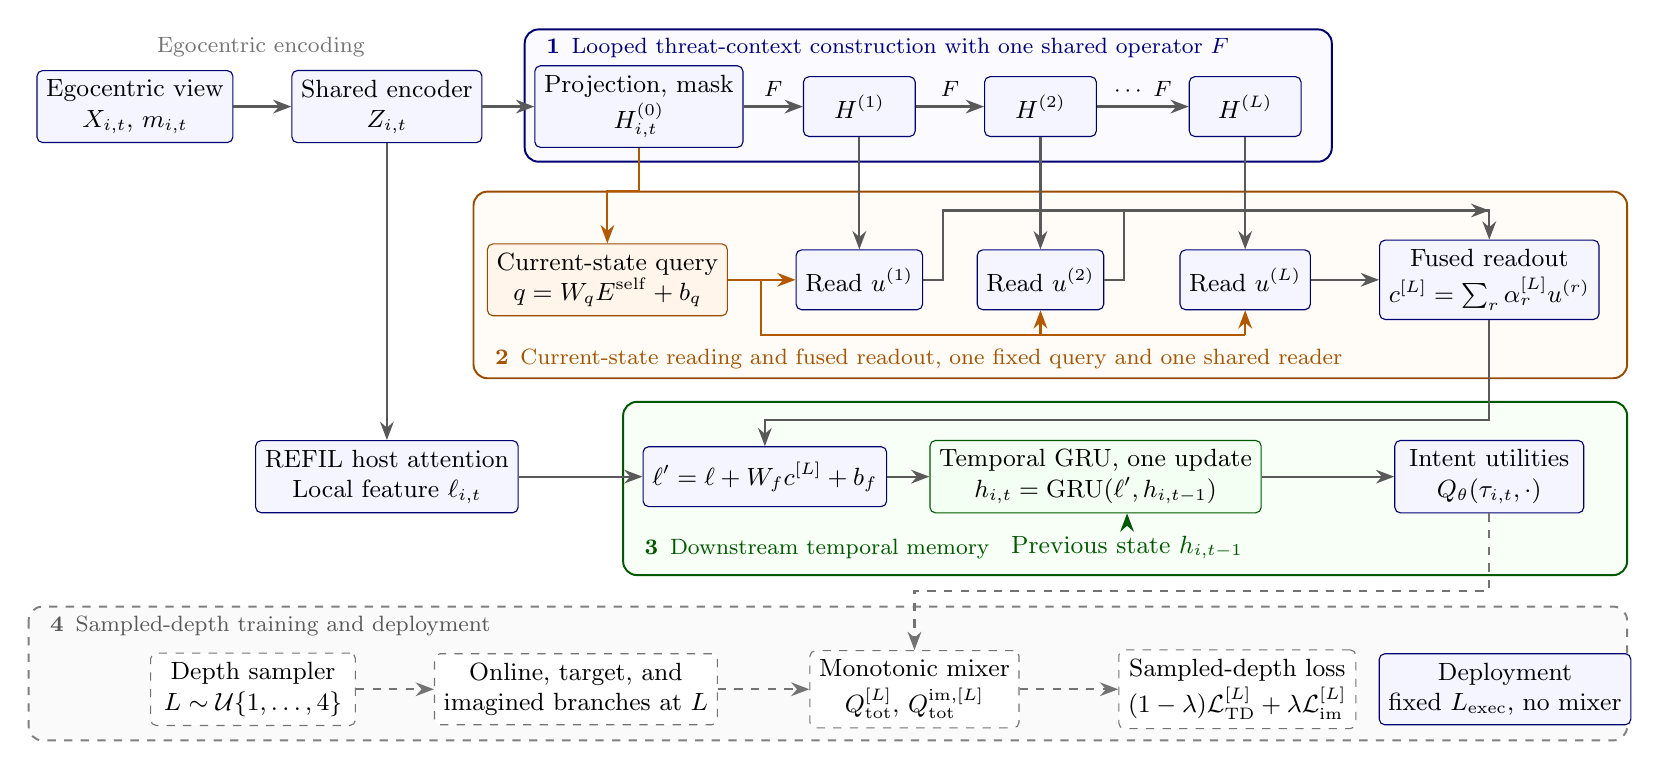
\begin{tikzpicture}[x=1cm,y=1cm,>=Stealth,
 box/.style={draw=blue!45!black,rounded corners=2pt,fill=blue!4,align=center,font=\small,minimum height=.76cm},
 smallbox/.style={box,minimum width=1.42cm},
 trainbox/.style={box,dashed,draw=black!55,fill=white},
 flow/.style={->,thick,draw=black!65},
 queryflow/.style={->,thick,draw=orange!70!black},
 trainflow/.style={->,thick,dashed,draw=black!55},
 frame/.style={rounded corners=5pt,line width=.7pt},
 tag/.style={anchor=west,font=\footnotesize},
 every node/.style={font=\small}]
\draw[frame,draw=blue!45!black,fill=blue!2] (4.95,-0.7) rectangle (15.2,0.98);
\draw[frame,draw=orange!60!black,fill=orange!3] (4.3,-1.08) rectangle (18.95,-3.45);
\draw[frame,draw=green!35!black,fill=green!3] (6.2,-3.75) rectangle (18.95,-5.95);
\draw[frame,dashed,draw=black!50,fill=black!2] (-1.35,-6.35) rectangle (18.95,-8.05);
\node[tag,text=blue!50!black] at (5.1,0.74) {\textbf{1}\enspace Looped threat-context construction with one shared operator $F$};
\node[tag,text=orange!65!black] at (4.45,-3.2) {\textbf{2}\enspace Current-state reading and fused readout, one fixed query and one shared reader};
\node[tag,text=green!35!black] at (6.35,-5.62) {\textbf{3}\enspace Downstream temporal memory};
\node[tag,text=black!65] at (-1.2,-6.6) {\textbf{4}\enspace Sampled-depth training and deployment};
\node[font=\footnotesize,text=black!55] at (1.6,0.76) {Egocentric encoding};
\node[box,minimum width=2.0cm] (obs) at (0,0) {Egocentric view\\$X_{i,t}$, $m_{i,t}$};
\node[box,minimum width=1.9cm] (enc) at (3.2,0) {Shared encoder\\$Z_{i,t}$};
\node[box,minimum width=1.7cm] (h0) at (6.4,0) {Projection, mask\\[2pt]$H^{(0)}_{i,t}$};
\node[smallbox] (h1) at (9.2,0) {$H^{(1)}$};
\node[smallbox] (h2) at (11.5,0) {$H^{(2)}$};
\node[smallbox] (hl) at (14.1,0) {$H^{(L)}$};
\draw[flow] (obs) -- (enc);
\draw[flow] (enc) -- (h0);
\draw[flow] (h0) -- node[above,font=\footnotesize] {$F$} (h1);
\draw[flow] (h1) -- node[above,font=\footnotesize] {$F$} (h2);
\draw[flow] (h2) -- node[above,font=\footnotesize] {$\cdots\ F$} (hl);
\node[box,fill=orange!8,draw=orange!60!black,minimum width=2.5cm] (query) at (6.0,-2.2) {Current-state query\\$q=W_qE^{\mathrm{self}}+b_q$};
\node[smallbox] (u1) at (9.2,-2.2) {Read $u^{(1)}$};
\node[smallbox] (u2) at (11.5,-2.2) {Read $u^{(2)}$};
\node[smallbox] (ul) at (14.1,-2.2) {Read $u^{(L)}$};
\node[box,minimum width=2.6cm] (fusion) at (17.2,-2.2) {Fused readout\\[2pt]$c^{[L]}=\sum_r\alpha^{[L]}_r u^{(r)}$};
\draw[queryflow] (h0.south) -- ++(0,-.55) -| (query.north);
\draw[flow] (h1) -- (u1);
\draw[flow] (h2) -- (u2);
\draw[flow] (hl) -- (ul);
\draw[queryflow] (query.east) -- (u1.west);
\draw[draw=orange!70!black,thick] (7.95,-2.2) -- (7.95,-2.9) -- (14.1,-2.9);
\draw[queryflow] (11.5,-2.9) -- (u2.south);
\draw[queryflow] (14.1,-2.9) -- (ul.south);
\draw[flow] (ul) -- (fusion);
\draw[flow] (u1.east) -- ++(.25,0) |- (17.2,-1.32) -- (fusion.north);
\draw[flow] (u2.east) -- ++(.25,0) |- (17.2,-1.32);
\node[box,minimum width=2.3cm] (base) at (3.2,-4.7) {REFIL host attention\\Local feature $\ell_{i,t}$};
\node[box,minimum width=2.45cm] (res) at (8.0,-4.7) {$\ell'=\ell+W_f c^{[L]}+b_f$};
\node[box,fill=green!5,draw=green!35!black,minimum width=2.8cm] (gru) at (12.2,-4.7) {Temporal GRU, one update\\$h_{i,t}=\operatorname{GRU}(\ell',h_{i,t-1})$};
\node[box,minimum width=2.4cm] (qval) at (17.2,-4.7) {Intent utilities\\$Q_\theta(\tau_{i,t},\cdot)$};
\draw[flow] (enc.south) -- (base.north);
\draw[flow] (base) -- (res);
\draw[flow] (fusion.south) |- (8.0,-3.98) -- (res.north);
\draw[flow] (res) -- (gru);
\draw[flow] (gru) -- (qval);
\node[font=\small,text=green!35!black] (prev) at (12.6,-5.6) {Previous state $h_{i,t-1}$};
\draw[flow,draw=green!35!black] (prev.north) -- (prev.north |- gru.south);
\node[trainbox,minimum width=2.6cm] (samp) at (1.5,-7.4) {Depth sampler\\$L\sim\mathcal U\{1,\dots,4\}$};
\node[trainbox,minimum width=2.6cm] (branch) at (5.6,-7.4) {Online, target, and\\imagined branches at $L$};
\node[trainbox,minimum width=2.6cm] (mix) at (9.9,-7.4) {Monotonic mixer\\[2pt]$Q^{[L]}_{\mathrm{tot}}$, $Q^{\mathrm{im},[L]}_{\mathrm{tot}}$};
\node[trainbox,minimum width=2.6cm] (loss) at (14.0,-7.4) {Sampled-depth loss\\[2pt]$(1-\lambda)\mathcal L^{[L]}_{\mathrm{TD}}+\lambda\mathcal L^{[L]}_{\mathrm{im}}$};
\node[box,minimum width=2.4cm] (deploy) at (17.4,-7.4) {Deployment\\fixed $L_{\mathrm{exec}}$, no mixer};
\draw[trainflow] (samp) -- (branch);
\draw[trainflow] (branch) -- (mix);
\draw[trainflow] (mix) -- (loss);
\draw[trainflow] (qval.south) |- (9.9,-6.15) -- (mix.north);
\end{tikzpicture}
}
\caption{Overview of LEAF at one decision of defender $i$. A shared encoder maps the egocentric entity view to tokens that feed the REFIL host path and the relational path. Module~1 initializes the context states $H^{(0)}$ from the current entities and refines them for $L$ rounds with one shared operator $F$. Module~2 reads every round with a fixed query formed from the defender's current self token and fuses the reads into the threat-context feature $c^{[L]}$. Module~3 adds $c^{[L]}$ to the host feature, and the temporal GRU then produces the intent utilities. The GRU state is the only quantity that persists across decision steps. Module~4 samples $L$ from one to four during training and applies the same depth to the online, target, and imagined branches. Deployment fixes $L$ as a compute budget and runs without the mixer.}
\label{fig:framework}
\end{figure*}

\subsection{Framework Overview}
\label{subsec:method-overview}
LEAF instantiates the utility network $Q_\theta$ of Section~\ref{subsec:pf-generalization} on top of REFIL~\cite{iqbal2021refil}. It rests on one observation. A defender's decision separates into three steps that draw on different information. Building the threat context draws only on the current entities, interpreting it for one defender adds only that defender's current state, and only inferring the hidden intent of the attackers needs history. LEAF gives each step its own module and lets history enter last. A fourth module trains the context builder so that it works at any depth.

Fig.~\ref{fig:framework} shows one decision of defender $i$. A shared encoder embeds the egocentric entity view, and the host path of REFIL pools it into a local feature. Module~1 refines the entity states for $L$ rounds with one shared attention operator. Module~2 reads every round with a query formed from the defender's current self token and fuses the reads into a threat-context feature. Module~3 adds this feature to the host feature and passes the sum to a gated recurrent unit (GRU), which outputs the intent utilities. The loop restarts from the current observation at every decision, and only the GRU state carries memory across decisions. During training, Module~4 samples $L$, and the mixer of \eqref{eq:fw-mixing} combines the utilities into a team value. At deployment, the mixer is dropped and $L$ becomes a compute budget. Algorithm~\ref{alg:leaf} lists the procedure.

All parameters are shared across entities, defenders, and rounds, and every map acts on each entity separately or combines entities through masked attention. LEAF therefore accepts any number of entities, does not depend on their order~\cite{lee2019settransformer}, and needs neither a population-specific parameter nor an explicit population count. This meets the set-structured requirement of Section~\ref{subsec:pf-requirements}. Modules~1 to~3 meet its other two requirements, and Module~4 answers the depth question raised in the Introduction.

\begin{algorithm}[!t]
\caption{LEAF Decision and Sampled-Depth Training}
\label{alg:leaf}
\begin{algorithmic}[1]
\REQUIRE Actor and mixer parameters $\Theta$, target copy $\bar\Theta$, replay buffer $\mathcal D$, maximum depth $L_{\max}$, weight $\lambda$
\STATE \textbf{Decision} of defender $i$ at step $t$ with depth $L$:
\STATE Compute $Z_{i,t}$, $\ell_{i,t}$, $E_{i,t}$, and $H^{(0)}_{i,t}$ by \eqref{eq:encoding}
\STATE $q_{i,t}\gets W_qE^{\mathrm{self}}_{i,t}+b_q$
\FOR{$r=1$ \TO $L$}
\STATE $H^{(r)}_{i,t}\gets F^{m_{i,t}}(H^{(r-1)}_{i,t})$ by \eqref{eq:loop} \COMMENT{Module 1}
\STATE Read $u^{(r)}_{i,t}$ with the fixed query by \eqref{eq:read} \COMMENT{Module 2}
\ENDFOR
\STATE Fuse the reads into $c^{[L]}_{i,t}$ by \eqref{eq:fusion} \COMMENT{Module 2}
\STATE Update $h_{i,t}$ and output $Q_\theta(\tau_{i,t},\cdot)$ by \eqref{eq:decision} \COMMENT{Module 3}
\STATE \textbf{Training} \COMMENT{Module 4}
\FOR{each collection round}
\STATE Draw $L_k\sim\mathcal U\{1,\dots,L_{\max}\}$ for each episode $k$
\STATE Run each episode $k$ with $\epsilon$-greedy decisions at depth $L_k$ and store it in $\mathcal D$
\FOR{each gradient step}
\STATE Sample a minibatch and $L\sim\mathcal U\{1,\dots,L_{\max}\}$
\STATE Unroll the online, target, and imagined branches with $L$ rounds
\STATE Update $\Theta$ by a gradient step on \eqref{eq:loss} at depth $L$
\ENDFOR
\STATE Copy $\Theta$ to $\bar\Theta$ at a fixed interval
\ENDFOR
\STATE \textbf{Deployment:} freeze $\Theta$, choose $L_{\mathrm{exec}}$, and act greedily without the mixer
\end{algorithmic}
\end{algorithm}

\subsection{Looped Threat-Context Construction}
\label{subsec:method-loop}
Defender $i$ arranges its observation $o_{i,t}$ as a matrix $X_{i,t}\in\mathbb R^{M\times d_x}$ with one row per entity and its own token first. The self row keeps the absolute position and velocity of the defender, and the other rows give positions and velocities relative to it, which exposes distances and closing motion directly. The mask $m_{i,t}\in\{0,1\}^{M}$ marks destroyed aircraft and padding rows, which never serve as attention keys and whose states $\operatorname{Mask}_{m}(\cdot)$ sets to zero. A rowwise encoder $\phi_{\mathrm{enc}}$, an affine map with a rectified linear unit, feeds both paths:
\begin{align}
Z_{i,t}&=\phi_{\mathrm{enc}}(X_{i,t}),\qquad \ell_{i,t}=\phi_{\mathrm{host}}(Z_{i,t},m_{i,t}),\nonumber\\
E_{i,t}&=\operatorname{Lin}_{g}(Z_{i,t}),\qquad H^{(0)}_{i,t}=\operatorname{Mask}_{m_{i,t}}(E_{i,t}).
\label{eq:encoding}
\end{align}
Here $\phi_{\mathrm{host}}$ is the self-query entity attention of REFIL with its output projection, $\operatorname{Lin}_{g}$ maps each token to the working width $d$, and $E^{\mathrm{self}}_{i,t}$ is the self row of $E_{i,t}$.

Module~1 refines the context states with one operator $F$ applied $L$ times, $H^{(r)}_{i,t}=F^{m_{i,t}}(H^{(r-1)}_{i,t})$. Omitting $i$ and $t$, one round is the residual attention block
\begin{align}
\widetilde H^{(r)}&=H^{(r-1)}+\operatorname{MHA}^{m}_{\mathrm c}\big(\operatorname{LN}_a(H^{(r-1)}),H^{(r-1)},H^{(r-1)}\big),\nonumber\\
H^{(r)}&=\operatorname{Mask}_{m}\big[\widetilde H^{(r)}+\operatorname{FFN}_{\mathrm c}\big(\operatorname{LN}_f(\widetilde H^{(r)})\big)\big],
\label{eq:loop}
\end{align}
where $\operatorname{MHA}^{m}_{\mathrm c}$ is multihead attention~\cite{vaswani2017attention} over queries, keys, and values with $-\infty$ logits at excluded keys, and layer normalization and the two-layer feedforward network act on each row. The defender's own token takes part in the context like any other teammate.

The context is built before it is read because of a property shared by every read over individually embedded entities, such as the reads of REFIL and SPECTra~\cite{iqbal2021refil,park2026spectra} or a read of $H^{(0)}$.

\begin{proposition}[Selection without context]
\label{prop:selection}
Let each row $z_j$ of $Z$ depend only on entity $j$ and defender $i$, and consider the read $u=\operatorname{MHA}^{m}(q,Z,Z)$. In every head, two permitted entities $a$ and $b$ receive attention weights with $w_a/w_b=\exp(s_a-s_b)$, where $s_j$ depends only on $q$ and $z_j$. The ratio is therefore identical in any two scenes that share $q$, $z_a$, and $z_b$, whatever the other entities are.
\end{proposition}

\begin{IEEEproof}
A head assigns $w_j=\exp(s_j)/\sum_k\exp(s_k)$, with $s_j=\langle W_Qq,W_Kz_j\rangle/\sqrt{d_{\mathrm k}}$ for key width $d_{\mathrm k}$ and the sum over permitted entities, so the normalizer cancels in $w_a/w_b$.
\end{IEEEproof}

Moving teammates toward or away from the targets of two attackers thus cannot change how such a read weighs one attacker against the other, and any dependence on coverage must be recovered later from the pooled vector. The ablation that reads $H^{(0)}$ in Section~\ref{sec:experiments} tests this restriction directly. A read of $H^{(L)}$ with $L\ge1$ is free of it, because by \eqref{eq:loop} every context state depends on all permitted entities. After one round, a target token can carry the teammates around it and an attacker token the target it approaches. After two, the attacker token can absorb the coverage-aware target token, so two rounds suffice for information to travel from teammate to target to attacker.

Sharing $F$ across rounds makes depth a free variable of one computation. The parameter count does not depend on $L$, and every sampled depth trains the same operator on both the initial tokens and its own outputs, as with the shared transition of Universal Transformers~\cite{dehghani2019universal}. Training thus favors a transformation that stays useful when applied to its own output, which is what execution at a different depth requires.

\subsection{Current-State Reading and Fused Readout}
\label{subsec:method-read}
Module~2 reads the context with a query formed from the defender's current self token, $q_{i,t}=W_qE^{\mathrm{self}}_{i,t}+b_q$, fixed for all rounds of the decision. A reader with its own parameters, shared across rounds, produces one read per round,
\begin{equation}
u^{(r)}_{i,t}=\operatorname{MHA}^{m_{i,t}}_{\mathrm r}\big(q_{i,t},H^{(r)}_{i,t},H^{(r)}_{i,t}\big),\quad r=1,\dots,L.
\label{eq:read}
\end{equation}
The query carries the defender's own state and previous intent, so a free defender and one engaged elsewhere can attend to different threats in the same scene. Because it ignores the loop states, every round answers the same question about a progressively refined context. It also ignores the temporal state, which Module~3 places downstream.

A linear scorer shared across rounds fuses the reads into the threat-context feature
\begin{align}
\zeta_r&=w_s^{\top}u^{(r)}_{i,t}+b_s,\qquad
\alpha^{[L]}_{r}=\frac{\exp(\zeta_r)}{\sum_{k=1}^{L}\exp(\zeta_k)},\nonumber\\
c^{[L]}_{i,t}&=\sum_{r=1}^{L}\alpha^{[L]}_{r}\,u^{(r)}_{i,t}.
\label{eq:fusion}
\end{align}
Because the scorer sees one read at a time, it serves any number of rounds, and the fusion weights still vary with the defender and the scene. Every depth $L$ yields its own feature $c^{[L]}_{i,t}$, so stopping after any round, which we call an exit, gives a complete decision feature built from the same weights. As in jumping knowledge networks~\cite{xu2018jk}, a deeper exit keeps the early reads while adding refinement, and the feature never relies on the last round alone, whose token states repeated attention can homogenize~\cite{dong2021attention}. All $L$ rounds are computed, and the weights decide only how their reads are combined.

\subsection{Downstream Temporal Memory}
\label{subsec:method-memory}
Module~3 adds the threat-context feature to the host feature and only then lets the temporal state enter:
\begin{align}
\ell'_{i,t}&=\ell_{i,t}+W_fc^{[L]}_{i,t}+b_f,\nonumber\\
h_{i,t}&=\operatorname{GRU}(\ell'_{i,t},h_{i,t-1}),\qquad
Q_\theta(\tau_{i,t},\cdot)=W_oh_{i,t}+b_o.
\label{eq:decision}
\end{align}
The zero-initialized projection $W_f,b_f$ lets training start from the host computation. The GRU updates once per decision, starts every episode from zero~\cite{hausknecht2015drqn}, and integrates the motion that reveals the private assignment of the attackers. At deployment, each defender selects the intent with the highest utility, and coordination arises from these intents without any assignment output.

For a fixed observation, mask, and depth, neither the query nor any quantity in \eqref{eq:encoding} to \eqref{eq:fusion} depends on $h_{i,t-1}$, so
\begin{equation}
\frac{\partial c^{[L]}_{i,t}}{\partial h_{i,t-1}}=0.
\label{eq:isolation}
\end{equation}
History shapes the utilities through the GRU and never changes how the current scene is built or read. A recurrent state accumulated in a large engagement can leave the range of states seen in small training engagements, and Section~\ref{sec:experiments} measures this drift. If such a state entered the query or the entity tokens, as the recurrent token of UPDeT and TransfQMix does~\cite{hu2021updet,transfqmix2023}, it would change which entities the defender attends to. Under \eqref{eq:isolation}, the threat-context feature depends on the present observation alone.

\subsection{Sampled-Depth Training and Deployment}
\label{subsec:method-training}
Module~4 trains the actor through the learning interface of REFIL. The mixer $f_{\mathrm{mix}}$ of \eqref{eq:fw-mixing} uses attention-based hypernetworks over the entity table~\cite{iqbal2021refil}. For each training sequence, REFIL also draws a random entity partition and forms within-group and cross-group masked views, whose auxiliary team value $Q^{\mathrm{im}}_{\mathrm{tot}}$ shares the target of the main branch. LEAF applies these masks to both feature paths. With team values $Q^{[L]}_{\mathrm{tot}}$ and $Q^{\mathrm{im},[L]}_{\mathrm{tot}}$ computed with $L$ rounds, LEAF minimizes
\begin{equation}
\mathcal L(\Theta)=\mathbb E_{L\sim\mathcal U\{1,\dots,L_{\max}\}}\Big[(1-\lambda)\,\mathcal L^{[L]}_{\mathrm{TD}}+\lambda\,\mathcal L^{[L]}_{\mathrm{im}}\Big],
\label{eq:loss}
\end{equation}
where $\mathcal L^{[L]}_{\mathrm{TD}}$ and $\mathcal L^{[L]}_{\mathrm{im}}$ are the mean squared errors of the two team values with respect to the target
\begin{equation}
y^{[L]}_t=r_t+\gamma\,\bar Q^{[L]}_{\mathrm{tot}}\big(s_{t+1},\mathbf a^{\star}_{t+1}\big).
\label{eq:target}
\end{equation}
Here $\Theta$ holds the actor parameters $\theta$ and the mixer parameters, $r_t$ is the training reward derived from \eqref{eq:fw-reward}, $\bar Q_{\mathrm{tot}}$ is the target network with parameters $\bar\Theta$, and $\mathbf a^{\star}_{t+1}$ collects the greedy intents of the online utilities. The bootstrap term is zero after natural termination, and we set $L_{\max}=4$ and $\lambda=0.5$.

Each parallel environment draws $L$ when an episode starts and keeps it for the episode, so the temporal state evolves under one consistent policy. Each minibatch draws one $L$ for its online, target, and imagined branches, so every temporal-difference error compares values from the same computation. Because Q-learning is off-policy, the two draws can be independent.

Every sampled depth supervises a complete policy. A shallow exit must already support good decisions, and a deeper exit must support them as well, so later rounds cannot undo what the first rounds built. Training at a fixed depth gives shallower exits no such signal. Sampled depth thus applies the idea of stochastic depth, LayerDrop, and early-exit training~\cite{huang2016stochastic,fan2020layerdrop,teerapittayanon2016branchynet,kaya2019overthinking} to the number of applications of one shared operator.

At deployment, LEAF freezes $\Theta$, drops the mixer, and runs $L_{\mathrm{exec}}$ rounds. One round costs $O(M^2d+Md^2)$ for each defender, so computation grows linearly with $L_{\mathrm{exec}}$ while the parameter count stays fixed, and the execution depth becomes a compute budget that needs no retraining. All experiments use $d_z=128$, $d=d_h=64$, four heads in every attention module, a feedforward width of $2d$, and $L_{\mathrm{exec}}=4$ unless stated otherwise. The next property states when a change of this budget keeps the decisions.

\begin{proposition}[Prefix-fusion stability]
\label{prop:prefix}
Fix one decision of defender $i$ at step $t$, including its observation and entering temporal state, and compare depths $p<L$. Let
\begin{equation*}
\beta=\sum_{r=p+1}^{L}\alpha^{[L]}_{r},\qquad
\xi=\max_{p<r\le L}\big\|u^{(r)}_{i,t}-c^{[p]}_{i,t}\big\|
\end{equation*}
be the fusion mass beyond round $p$ and the largest distance from a later read to the depth-$p$ feature. Then
\begin{equation}
\big\|c^{[L]}_{i,t}-c^{[p]}_{i,t}\big\|\le\beta\xi.
\label{eq:prefix}
\end{equation}
Let $\delta$ be the largest change of any utility $Q_\theta(\tau_{i,t},a)$ between the two depths. Depth $p$ selects the same greedy intent as depth $L$ whenever the depth-$L$ utility gap between the best and the second-best intents exceeds $2\delta$. If the map from $c$ to $Q_\theta(\tau_{i,t},\cdot)$ defined by \eqref{eq:decision} is $\kappa$-Lipschitz on the segment between $c^{[p]}_{i,t}$ and $c^{[L]}_{i,t}$, from the norm in $\xi$ to the max norm, then $\delta\le\kappa\beta\xi$.
\end{proposition}

\begin{IEEEproof}
The first $p$ rounds do not depend on $L$, so the reads and scores up to round $p$ coincide at both depths, and $\alpha^{[p]}_{r}=\alpha^{[L]}_{r}/(1-\beta)$ for $r\le p$. Hence
\begin{equation*}
c^{[L]}-c^{[p]}=\sum_{r=p+1}^{L}\alpha^{[L]}_{r}\big(u^{(r)}-c^{[p]}\big),
\end{equation*}
and the triangle inequality gives \eqref{eq:prefix}. If the best intent at depth $L$ leads every other intent by more than $2\delta$, it still leads at depth $p$, since each utility moves by at most $\delta$. The host feature and the entering temporal state are common to both depths, so the utilities differ only through $c$, and the Lipschitz condition with \eqref{eq:prefix} gives $\delta\le\kappa\beta\xi$.
\end{IEEEproof}

The bound holds for every $p<L$, including $L>L_{\max}$, so it covers both truncating the loop and extending it beyond the training range. When the readout places little mass beyond round $p$ and the late reads stay near the early fused feature, changing the depth barely moves the threat-context feature and keeps every decision with a clear utility gap. Section~\ref{sec:experiments} measures this fusion mass and checks the condition on recorded decisions.


% =====================================================================
% Section V (Experiments) of the 1015 draft, input from Papers/1015/main.tex.
% Defines: sec:experiments, subsec:exp-setup, subsec:exp-comparison, subsec:exp-ablation,
%   subsec:exp-mechanism, tab:exp-scales, tab:exp-methods, tab:exp-main, tab:exp-ablation,
%   fig:exp-generalization, fig:exp-capacity, fig:exp-memory, fig:exp-depth.
% Uses: subsec:pf-scenario, subsec:pf-decpomdp, subsec:pf-attacker, eq:fw-reward (Section III),
%   sec:method, subsec:method-loop, subsec:method-memory, subsec:method-training, prop:selection,
%   prop:prefix (Section IV).
% Packages already loaded by main.tex: booktabs, multirow, graphicx.
% New references: listed in sections/sec_5_6/references_sec5_6.bib and merged into Papers/1015/references.bib.
% Figures: figures/exp_*.pdf, rendered by figures/src/figures.py from Open-SCORE/outputs/main.
%   Table rows: python figures/src/figdata.py --tables.
% Vehicle model: kept generic. Dynamics and engagement constants appear only in Section III.
% =====================================================================

\section{Experiments}
\label{sec:experiments}

This section answers three questions. Does a policy trained once on small engagements protect targets better than existing methods when it is deployed at larger scales? Which designs of LEAF produce this generalization? Why do these designs work? Section~\ref{subsec:exp-setup} describes the setup, and Sections~\ref{subsec:exp-comparison} to~\ref{subsec:exp-mechanism} answer the three questions in turn.

\begin{table}[!t]
\centering
\footnotesize
\setlength{\tabcolsep}{4pt}
\caption{Scale protocol. Configurations are written $(N,K)$ with $N=N_R=N_B$.}
\label{tab:exp-scales}
\begin{tabular}{@{}llc@{}}
\toprule
Set & Configurations $(N,K)$ & Count\\
\midrule
Training & $N\in\{4,6,8,10\}$, $K\in\{1,2,3\}$, drawn per episode & --\\
ID & (4,2), (6,2), (8,2), (10,3) & 4\\
$K$-OOD & (10,4), (10,6), (10,9), (10,12) & 4\\
$N$-OOD & (15,2), (20,2), (25,2), (30,2), (40,2), (50,2) & 6\\
\multirow{2}{*}{Joint-OOD} & (15,4), (15,6), (20,4), (20,6), & \multirow{2}{*}{8}\\
 & (30,4), (30,6), (30,9), (30,12) & \\
Extra & (5,2), (10,2) & 2\\
\bottomrule
\end{tabular}
\vspace{2pt}

\parbox{\columnwidth}{\footnotesize Every evaluation configuration uses the same 300 initial scenes for all methods. The two extra configurations enter only the scale sweeps of Fig.~\ref{fig:exp-generalization} and the averages over all 24 configurations.}
\end{table}

\begin{table}[!t]
\centering
\footnotesize
\setlength{\tabcolsep}{3pt}
\caption{Compared methods. Parameters count the networks used at deployment.}
\label{tab:exp-methods}
\begin{tabular}{@{}l p{0.53\columnwidth} c r@{}}
\toprule
Method & Coordination mechanism & Target & Params\\
\midrule
QMIX & Self-query entity attention, monotonic entity mixer & DQ & 102k\\
REFIL & QMIX with randomly grouped imagined entity views & DQ & 102k\\
DCG & Utilities and pairwise payoffs on a complete coordination graph & DQ & 112k\\
ALMA & Learned target allocation and allocation-conditioned actor & DQ & 283k\\
TransfQMix & Transformer actor and mixer with a memory token & TD($\lambda$) & 51k\\
SPECTra & Typed set projections, self-query read, set mixer & TD($\lambda$) & 47k\\
Rule & Integer assignment with predicted interception at every step & -- & --\\
LEAF & Looped threat context on the REFIL host & DQ & 176k\\
\bottomrule
\end{tabular}
\vspace{2pt}

\parbox{\columnwidth}{\footnotesize DQ denotes one-step double Q-learning with RMSprop, and TD($\lambda$) denotes $\lambda$-returns with Adam, as in the original implementations. All learned methods carry recurrent memory.}
\end{table}

\begin{table*}[!t]
\centering
\footnotesize
\setlength{\tabcolsep}{3.4pt}
\caption{Zero-shot results on the four test groups. Damage $D$ gives the mean and SD over three training seeds, and $P$ and CVaR give seed means. The best value in each column is in bold and the second best is underlined.}
\label{tab:exp-main}
\begin{tabular}{@{}l cccc c cccc c cccc@{}}
\toprule
& \multicolumn{4}{c}{Damage $D\downarrow$} && \multicolumn{4}{c}{Damage incidence $P$ (\%)\,$\downarrow$} && \multicolumn{4}{c}{Tail damage CVaR\,$\downarrow$}\\
\cmidrule{2-5}\cmidrule{7-10}\cmidrule{12-15}
Method & ID & $K$-OOD & $N$-OOD & Joint && ID & $K$-OOD & $N$-OOD & Joint && ID & $K$-OOD & $N$-OOD & Joint\\
\midrule
QMIX & 2.32$\pm$1.43 & 5.01$\pm$2.50 & 5.14$\pm$3.11 & 7.42$\pm$3.97 && 82.1 & 92.9 & 92.0 & 94.4 && 5.18 & 10.94 & 11.57 & 15.98\\
REFIL & \underline{0.72}$\pm$0.05 & \underline{1.80}$\pm$0.30 & 2.21$\pm$0.28 & 3.31$\pm$0.30 && \underline{44.4} & \underline{60.4} & \underline{67.0} & \underline{73.2} && \underline{2.79} & \underline{6.18} & 7.81 & 10.66\\
DCG & 2.03$\pm$0.44 & 5.84$\pm$1.92 & 5.02$\pm$2.66 & 8.09$\pm$3.91 && 85.2 & 96.4 & 94.8 & 97.9 && 4.99 & 12.07 & 11.77 & 17.32\\
ALMA & 1.33$\pm$0.19 & 3.02$\pm$0.34 & 3.61$\pm$0.74 & 5.37$\pm$1.04 && 67.8 & 83.0 & 90.3 & 92.6 && 3.86 & 7.78 & 9.10 & 12.97\\
TransfQMix & 1.53$\pm$0.28 & 3.95$\pm$0.50 & 4.02$\pm$0.97 & 6.63$\pm$1.20 && 68.5 & 88.1 & 89.5 & 93.9 && 4.39 & 9.63 & 10.84 & 15.87\\
SPECTra & 2.48$\pm$0.21 & 6.74$\pm$0.53 & 5.05$\pm$0.59 & 9.84$\pm$0.49 && 90.9 & 98.9 & 95.6 & 99.3 && 5.71 & 13.30 & 12.09 & 19.49\\
Rule$^\dagger$ & 1.46$\pm$0.72 & 3.21$\pm$1.13 & \underline{1.54}$\pm$0.88 & \underline{3.06}$\pm$0.98 && 80.2 & 92.6 & 75.1 & 88.9 && 3.77 & 7.15 & \underline{4.67} & \underline{7.70}\\
LEAF & \textbf{0.41}$\pm$0.10 & \textbf{1.00}$\pm$0.23 & \textbf{0.57}$\pm$0.23 & \textbf{1.10}$\pm$0.10 && \textbf{27.6} & \textbf{41.4} & \textbf{31.4} & \textbf{39.1} && \textbf{2.10} & \textbf{4.14} & \textbf{3.10} & \textbf{5.41}\\
\midrule
LEAF vs.\ best & $-$43\% & $-$45\% & $-$63\% & $-$64\% && $-$38\% & $-$31\% & $-$53\% & $-$47\% && $-$25\% & $-$33\% & $-$34\% & $-$30\%\\
\bottomrule
\end{tabular}
\vspace{2pt}

\parbox{\textwidth}{\footnotesize $^\dagger$Rule has no training seeds, and its SD is taken over scenes. Joint denotes Joint-OOD. CVaR is the mean damage of the worst 30 of the 300 episodes in each configuration. The last row compares LEAF with the best other method in each column.}
\end{table*}

\begin{figure*}[!t]
\centering
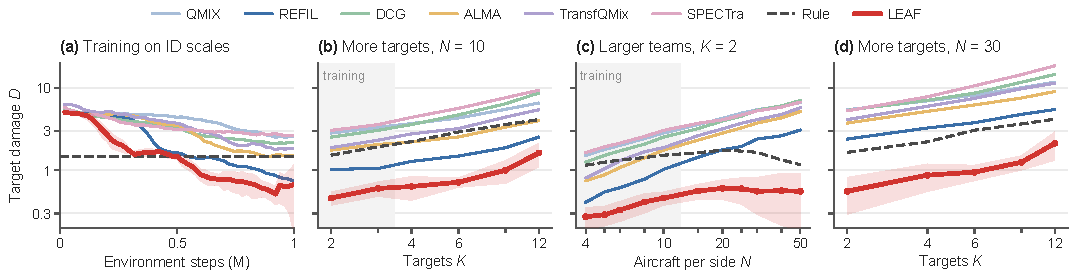
\includegraphics[width=\textwidth]{figures/exp_generalization.pdf}
\caption{Learning and zero-shot scale generalization. (a) Damage on the ID validation scenes during training, smoothed over five consecutive validation points. The dashed line marks the ID damage of Rule. (b)--(d) Damage of the frozen final policies as the number of targets grows at $N=10$, as the team grows at $K=2$, and as the number of targets grows at $N=30$, beyond the training team size. Gray shading marks the training range. Each point averages 300 common scenes and three training seeds, and the red band shows one SD of LEAF over the seeds. Table~\ref{tab:exp-main} lists the SDs of all methods.}
\label{fig:exp-generalization}
\end{figure*}

\subsection{Experimental Setup}
\label{subsec:exp-setup}

\emph{Task and scale protocol.} All experiments use the SkyHAD Damage task of Section~\ref{subsec:pf-scenario}. $N$ defenders protect $K$ stationary targets against $N$ attackers that follow the rule of Section~\ref{subsec:pf-attacker}, and an episode ends when all attackers are destroyed or after 100 decisions. During training, every episode draws its own configuration with $N\in\{4,6,8,10\}$ and $K\in\{1,2,3\}$. The frozen policies are then deployed on the configurations of Table~\ref{tab:exp-scales}. These form an in-distribution (ID) group and three out-of-distribution (OOD) groups that enlarge the number of targets, the team size, or both, which we call $K$-OOD, $N$-OOD, and Joint-OOD. Two extra configurations inside the training range complete the scale sweeps. The largest deployments have five times as many aircraft per side or four times as many targets as the largest training configuration. Training adds a potential-based shaping term to the team reward \eqref{eq:fw-reward}, which leaves the optimal policy unchanged~\cite{ng1999shaping}. All reported results use the unshaped episode damage.

\emph{Baselines.} We compare LEAF with six learned baselines and a rule-based controller, summarized in Table~\ref{tab:exp-methods}. Each represents one approach to scalable cooperative defense. QMIX~\cite{rashid2018qmix} and REFIL~\cite{iqbal2021refil} factorize the team value, and each defender reads the raw entities once with a query formed from its own state. We use QMIX in its entity-attention form with the entity mixer of REFIL. REFIL is the host of LEAF and thus its closest comparison. DCG~\cite{boehmer2020dcg} models pairwise coordination at the level of actions. ALMA~\cite{iqbal2022alma} first allocates defenders to targets and then maneuvers, the decomposition common in defense automation. TransfQMix~\cite{transfqmix2023} and SPECTra~\cite{park2026spectra} were designed for scalability. TransfQMix relates the entities and a memory token over several Transformer layers, and SPECTra encodes typed entity sets before a self-query read. Rule represents optimization-based engineering practice. At every step, it selects the attackers closest to the defenders, at most as many as there are living defenders, and solves a 0--1 integer program. The program assigns every defender to one selected attacker and covers every selected attacker while minimizing the total distance between the defenders and the attacker positions predicted one step ahead at constant velocity. Each defender then takes the acceleration intent closest to the velocity that intercepts its attacker. Like the attacker rule of Section~\ref{subsec:pf-attacker}, Rule separates assignment from steering.

\emph{Common adaptation.} All learned methods use the entity observation of Section~\ref{subsec:pf-decpomdp} with the same features and masks, the same intent set, the same attackers, the same training distribution, and $10^6$ environment steps per training run. Each method keeps its architecture and learning rule, and we replace only its input interface, action head, and masks. Each method also handles variable scale with its own mechanism. QMIX, REFIL, ALMA, and LEAF use the attention-based entity mixer of REFIL, SPECTra uses its set hypernetwork mixer, and TransfQMix uses its Transformer mixer. DCG builds a complete coordination graph over the deployed team, and ALMA treats each target as a subtask.

\emph{Training.} Every method is trained with three seeds. Eight parallel environments collect data, and each collection round is followed by eight updates on minibatches of 32 episodes from a replay buffer of 5000 episodes. All methods use a discount of 0.99, gradient clipping at 10, hard target updates every 200 episodes, and $\epsilon$-greedy exploration annealed from 1.0 to 0.05 over $10^5$ steps, or $5\times10^4$ steps for DCG. LEAF, QMIX, REFIL, DCG, and ALMA use RMSprop with a learning rate of $5\times10^{-4}$ and one-step double Q-learning targets~\cite{vanhasselt2016double}. SPECTra and TransfQMix keep Adam with a learning rate of $10^{-3}$ and $\lambda$-returns with $\lambda=0.6$ from their implementations. LEAF uses the architecture of Section~\ref{subsec:method-training}, samples $L$ uniformly from one to four during training, and executes $L_{\mathrm{exec}}=4$ rounds unless stated otherwise. Every $2\times10^4$ steps, each run is evaluated on the four ID configurations with 25 episodes each from a separate scene pool. These 50 validation points produce the learning curves and play no role in model selection.

\emph{Evaluation and metrics.} Evaluation is zero-shot. We take the final weights at the end of the budget, freeze them, select intents greedily, and apply no fine-tuning. Every model runs the same 300 initial scenes in every configuration. The attackers react to the defenders, so one initial scene can unfold differently under different policies, as closed-loop evaluation requires. The primary metric is the episode damage $D$ of Section~\ref{subsec:pf-decpomdp}, summed over all targets without capping. Two further metrics describe the quality of protection. The damage incidence $P$ is the fraction of episodes in which at least one target is damaged. The conditional value at risk (CVaR) is the mean damage of the worst 10\% of episodes in a configuration and measures tail risk. The mechanism analyses also report the fraction $I$ of attackers that are intercepted and the fraction $C$ of defenders lost to friendly collisions. For every trained model, we average over the scenes of a configuration and then over the configurations of a group with equal weight. We report the mean and the sample standard deviation (SD) over the three training seeds. Rule has no training seed, and its SD is taken over scenes. With three seeds per method, we state comparisons at the level of individual seeds, which readers can check directly~\cite{agarwal2021rliable}.

\begin{table*}[!t]
\centering
\footnotesize
\setlength{\tabcolsep}{2.5pt}
\caption{Single-factor ablations. Each row of the main chain changes one design of the row above, and each side row changes one design of the parent it names. Damage $D$ gives the mean and SD over three training seeds, with the change relative to the row above in parentheses. The best value in each column is in bold.}
\label{tab:exp-ablation}
\begin{tabular}{@{}cl l cc cccc@{}}
\toprule
& Variant & Change & Train $L$ & Query & ID & $K$-OOD & $N$-OOD & Joint-OOD\\
\midrule
0 & Direct read & Reads the raw entities $H^{(0)}$ & -- & memory & 0.93$\pm$0.21 & 1.96$\pm$0.46 & 2.02$\pm$0.45 & 3.20$\pm$0.69\\
1 & One round & Adds one context round & 1 & memory & 0.61$\pm$0.27 {\scriptsize($-$34\%)} & 1.20$\pm$0.40 {\scriptsize($-$39\%)} & 1.36$\pm$0.88 {\scriptsize($-$33\%)} & 2.16$\pm$1.01 {\scriptsize($-$33\%)}\\
2 & Fixed depth & Refines for four rounds & 4 & memory & 0.41$\pm$0.20 {\scriptsize($-$33\%)} & 1.00$\pm$0.66 {\scriptsize($-$17\%)} & 0.66$\pm$0.18 {\scriptsize($-$51\%)} & 1.27$\pm$0.23 {\scriptsize($-$41\%)}\\
3 & Memory query & Samples the training depth & 1--4 & memory & 0.53$\pm$0.23 {\scriptsize(+29\%)} & 1.53$\pm$0.73 {\scriptsize(+52\%)} & 1.00$\pm$0.62 {\scriptsize(+51\%)} & 1.95$\pm$1.23 {\scriptsize(+54\%)}\\
4 & \textbf{LEAF} & Moves memory out of the query & 1--4 & current & \textbf{0.41}$\pm$0.10 {\scriptsize($-$23\%)} & \textbf{1.00}$\pm$0.23 {\scriptsize($-$35\%)} & 0.57$\pm$0.23 {\scriptsize($-$42\%)} & \textbf{1.10}$\pm$0.10 {\scriptsize($-$44\%)}\\
\midrule
& Unshared rounds & Fixed depth, untied rounds & 4 & memory & 0.48$\pm$0.18 & 1.13$\pm$0.16 & \textbf{0.54}$\pm$0.16 & 1.23$\pm$0.25\\
& Last read & Memory query, last read only & 1--4 & memory & 0.43$\pm$0.08 & 1.02$\pm$0.10 & 0.65$\pm$0.16 & 1.27$\pm$0.20\\
& No host & Memory query, no REFIL host & 1--4 & memory & 0.51$\pm$0.14 & 1.77$\pm$0.62 & 1.26$\pm$0.65 & 2.32$\pm$0.89\\
& REFIL-matched & REFIL widened to 176k parameters & -- & -- & 0.91$\pm$0.17 & 2.49$\pm$0.28 & 2.27$\pm$0.31 & 4.17$\pm$0.76\\
\bottomrule
\end{tabular}
\vspace{2pt}

\parbox{\textwidth}{\footnotesize All variants execute four rounds except One round, which executes one, and Direct read and REFIL-matched, which have no context loop. A memory query adds the previous recurrent state, with a stopped gradient, to the current self token that forms the query.}
\end{table*}

\subsection{Zero-Shot Scale Generalization}
\label{subsec:exp-comparison}

We first ask whether a policy trained once on small engagements protects targets better than existing methods when it is deployed at larger scales. Table~\ref{tab:exp-main} and Fig.~\ref{fig:exp-generalization} answer this question.

LEAF has the lowest mean damage in all four groups and in each of the 24 evaluation configurations. Relative to the strongest competitor in each group, it reduces damage by 43\% in ID, 45\% under target-count extrapolation, 63\% under team-size extrapolation, and 64\% under joint extrapolation. The advantage holds for every training run. In every group, the worst of the three LEAF models incurs less damage than the best model of each learned baseline and than Rule. The ordering repeats on an independent pool of 300 scenes per configuration, where the damage averaged over all 24 configurations is 0.79 for LEAF, 2.09 for REFIL, 4.25 for TransfQMix, and 6.30 for SPECTra.

In Fig.~\ref{fig:exp-generalization}(c), the damage of LEAF stays between 0.56 and 0.61 as teams grow from 15 to 50 aircraft per side, whereas every learned baseline degrades steadily. The damage of REFIL, for example, rises from 1.44 to 3.08. More attackers create more combinations of attackers, targets, and teammates that a defender must tell apart. By Proposition~\ref{prop:selection}, a read of individually embedded entities weighs each attacker by its own features and the query, so it cannot favor an attacker because the attacker's target is unguarded. LEAF relates attackers to targets and teammates before any defender reads the scene, and its damage barely changes as the team grows. Rule solves its assignment anew at every scale and also stays nearly flat. Under team-size and joint extrapolation, it incurs less damage than every learned baseline. In Fig.~\ref{fig:exp-generalization}(b) and (d), more targets raise the damage of every method, because the attackers then have more targets to choose from. LEAF remains the lowest at every target count, and this holds when the team is already three times the training size.

The protection metrics in Table~\ref{tab:exp-main} show the same advantage at the level of episodes. LEAF keeps every target undamaged in 59\% to 72\% of episodes. No other method exceeds 56\% in any group, and Rule stays below 25\%. The mean damage of the worst 10\% of episodes is 25\% to 34\% lower for LEAF than for the strongest competitor in each group. Rule is the strongest competitor on average damage at large scales, yet it lets at least one target be damaged in 75\% to 93\% of episodes. Assigning attackers by distance gives every attacker a pursuer, but it cannot tell which attacker threatens an uncovered target. LEAF weighs each attacker by its threat context and leaves fewer targets exposed.

LEAF also learns faster. In Fig.~\ref{fig:exp-generalization}(a), its validation damage first falls below 1.0 after about $0.56\times10^6$ steps. REFIL needs about $0.86\times10^6$ steps, and no other learned baseline reaches this level within the budget.

\begin{figure}[!t]
\centering
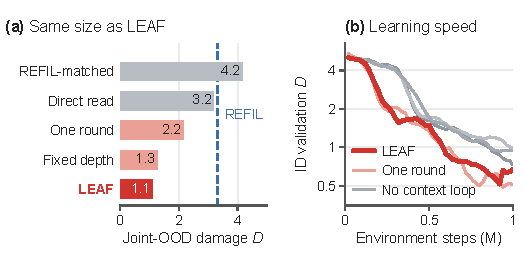
\includegraphics[width=\columnwidth]{figures/exp_capacity.pdf}
\caption{Organization versus size. (a) Joint-OOD damage of the models that share the size of LEAF, 176k parameters. Gray bars mark models that read the entities without a context loop, and red bars models that build the context in a loop. The dashed line marks REFIL, which has 102k parameters. (b) ID validation damage during training, smoothed over five validation points, with REFIL, REFIL-matched, and Direct read drawn in gray. All values are means over three training seeds.}
\label{fig:exp-capacity}
\end{figure}

\begin{figure}[!t]
\centering
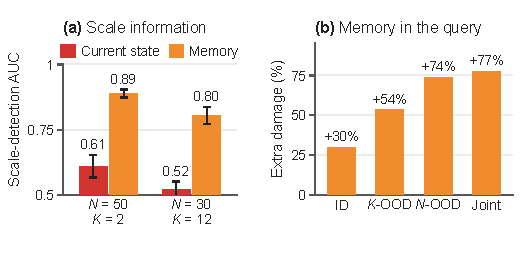
\includegraphics[width=\columnwidth]{figures/exp_memory.pdf}
\caption{Memory after reading. (a) AUC of a linear classifier that separates decisions in a shifted configuration from decisions at $(N,K)=(10,2)$, using either the current self features that form the query of LEAF or its recurrent state $h_{t-1}$. Bars start at the chance level of 0.5, and error bars show one SD over three training seeds. Each configuration contributes ten scenes per model. (b) Extra damage of Memory query, which feeds the recurrent state into the query, relative to LEAF in each group. Joint denotes Joint-OOD.}
\label{fig:exp-memory}
\end{figure}

\begin{figure*}[!t]
\centering
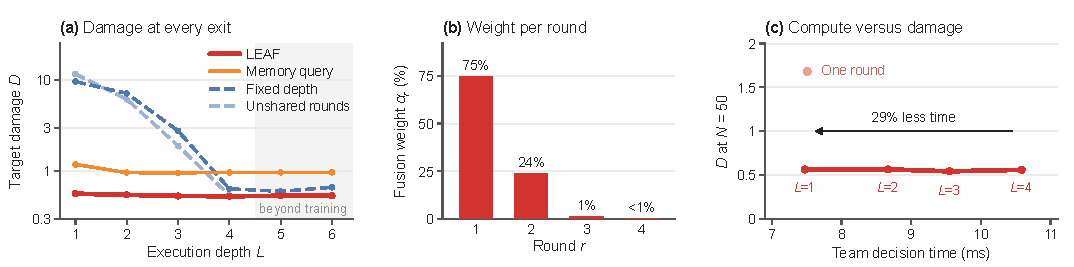
\includegraphics[width=\textwidth]{figures/exp_depth.pdf}
\caption{Execution at any depth. (a) Closed-loop damage at execution depths one to six, averaged over $(N,K)=(10,2)$, $(30,2)$, and $(50,2)$ with 300 scenes each and over three training seeds. Solid lines mark sampled-depth training and dashed lines training at four rounds only. Unshared rounds has no parameters beyond its fourth round, and LEAF comes from a separate depth evaluation with the same protocol. (b) Fusion weight of each round in normal four-round execution of LEAF, averaged over $(10,2)$, $(30,2)$, and $(30,12)$. (c) Full-team decision time and damage at $(50,2)$ for LEAF executed with one to four rounds and for One round. Times come from 20 closed-loop episodes on the workstation described in Section~\ref{subsec:exp-mechanism}, and damage values are means over three training seeds.}
\label{fig:exp-depth}
\end{figure*}

\subsection{Ablation Study}
\label{subsec:exp-ablation}

We next retrain variants of LEAF to identify which designs produce this generalization. All variants share the training budget, seeds, and evaluation of LEAF. Their saved configurations show that consecutive rows of the main chain in Table~\ref{tab:exp-ablation} differ in exactly one switch, so the chain adds the designs of Section~\ref{sec:method} one at a time. Direct read reads the raw entities $H^{(0)}$. One round builds the context for one round before reading, and Fixed depth refines it for four rounds with training at four rounds only. Memory query samples the training depth, and LEAF finally removes the recurrent state from the query. Every variant before LEAF feeds the previous recurrent state into the query with a stopped gradient, so the last step isolates the placement of memory.

Context construction is the foundation. A single context round removes 33\% to 39\% of the damage of Direct read in every group, with the query and training otherwise unchanged. Direct read is exactly the read that Proposition~\ref{prop:selection} restricts, so moving teammates toward or away from a target cannot shift its attention between attackers. After one round, each attacker token already carries information about the target it approaches and the teammates nearby, and the read can weigh attackers by their context.

Refining the context for four rounds lowers damage further, by 33\% in ID and by 51\% and 41\% under team-size and joint extrapolation, and all three seeds improve in both of these groups. In small engagements, one round already captures the relations that matter. With more entities, whether a target is covered depends on relations that a second round composes from the first, as Section~\ref{subsec:method-loop} explains. Multi-round refinement therefore pays off most when the scale grows.

Removing the recurrent state from the query lowers damage by 23\% in ID and by 35\% to 44\% in the extrapolation groups. Seen from LEAF, feeding memory into the query raises damage by 30\% in ID and by 54\% to 77\% under extrapolation, and the spread across seeds grows with it. Under joint extrapolation, the SD rises from 0.10 for LEAF to 1.23 for Memory query. Memory placement thus matters most where deployment departs furthest from training, and Section~\ref{subsec:exp-mechanism} traces this effect to drift of the recurrent state.

Sampling the training depth raises the four-round damage within the memory-query family, mostly through one of the three training runs. LEAF also samples its depth and matches or improves on Fixed depth in all four groups. The value of sampled depth lies in the shallower exits, which Section~\ref{subsec:exp-mechanism} examines. Untying the rounds in Unshared rounds or reading only the last round in Last read leaves the four-round damage close to that of LEAF, and these choices matter when the execution depth changes. Removing the REFIL host in No host raises damage in all three extrapolation groups, so LEAF builds on the entity grouping of its host.

\subsection{Mechanism Analysis}
\label{subsec:exp-mechanism}

Finally, we examine why LEAF works through three properties of its computation. The gain comes from how the computation is organized, reading the scene from the current state keeps its interpretation stable as memory drifts, and sampled-depth training makes every execution depth a usable policy.

\emph{Organization over size.} REFIL-matched widens the actor of REFIL with a residual multilayer perceptron to within 0.4\% of the parameter count of LEAF. Its damage is 2.3 to 3.9 times that of LEAF and higher than that of REFIL in all four groups. Fig.~\ref{fig:exp-capacity}(a) compares the models that share the size of LEAF. Their joint-extrapolation damage spans almost a factor of four, and every model that builds the context in a loop incurs less damage than REFIL. Size does not predict damage across methods either. ALMA has as many parameters as Unshared rounds and more than four times its joint-extrapolation damage. Context construction also speeds up learning. In Fig.~\ref{fig:exp-capacity}(b), One round learns at the pace of LEAF, whereas Direct read and REFIL-matched follow REFIL. The trained policy relies on this context. When the frozen LEAF policy reads the raw entities $H^{(0)}$ in place of its context, damage rises in all nine combinations of model and configuration that we tested, with ten scenes each.

\emph{Memory after reading.} Section~\ref{subsec:method-memory} argued that a recurrent state accumulated in a larger engagement can leave the range seen in training. We test this with a probe~\cite{alain2017probes}. For each training seed, a classifier separates decisions in a shifted configuration from decisions at $(N,K)=(10,2)$, using either the recurrent state $h_{t-1}$ of LEAF or the current self features from which its query is formed. In Fig.~\ref{fig:exp-memory}(a), a linear classifier identifies the deployment scale from the recurrent state with an area under the receiver operating characteristic curve (AUC) of 0.89 at $(50,2)$ and 0.80 at $(30,12)$. From the current self features it reaches only 0.61 and 0.52. Gradient-boosted trees give the same picture, and every seed agrees. Memory learned in small engagements thus moves into new regions as the scale grows, while the current self state stays close to the training distribution. The query is a deterministic function of the self features, so it carries no more scale information than they do.

Feeding memory into the query carries this drift into the reading of the scene. Fig.~\ref{fig:exp-memory}(b) shows that the extra damage of Memory query grows from 30\% in ID to 77\% under joint extrapolation, and Table~\ref{tab:exp-ablation} shows that its seeds spread further apart. Team behavior follows the same order. In the four configurations with protection records, Memory query lies between REFIL and LEAF on interception, damage incidence, tail damage, and friendly collisions in all 16 comparisons. Memory remains useful downstream. Resetting the recurrent state of the frozen LEAF policy at every step raises damage in eight of nine combinations of model and configuration. LEAF therefore keeps memory for selecting intents and keeps it out of the step that reads the threat context.

\emph{Every exit is a usable policy.} In normal four-round execution, the first two rounds receive about 99\% of the fusion weight in every configuration we examined, and the first round alone about three quarters, as Fig.~\ref{fig:exp-depth}(b) shows. The split varies across defenders, with an SD of 11 to 14 percentage points among the defenders of the same state, so each defender draws on the rounds in its own way. Proposition~\ref{prop:prefix} links this small fusion mass beyond the second round to stable decisions. We execute two rounds instead of four in the same states for 48{,}705 decisions at $(10,2)$, $(50,2)$, and $(30,12)$, with ten scenes per model. The greedy intent changes in only 1.1\% to 1.7\% of the decisions. For 79\% of them, the utility gap exceeds twice the largest utility change $\delta$ between the two depths, the condition of the proposition, so these decisions keep their intent. The decisions that do change lie mostly in the lowest tenth of utility gaps, 78\% to 81\% of them, where the two best intents are nearly equivalent.

Closed-loop execution confirms the same picture. Over all 24 configurations, executing two rounds instead of four changes the damage of LEAF by about 1\%, and a single round by about 2\%. Executing five or six rounds, beyond the training range, changes it by less than 0.1\%. Sampled-depth training is what keeps the shallow exits usable. Memory query and Fixed depth share the architecture and the query and differ only in how the training depth is chosen. In Fig.~\ref{fig:exp-depth}(a), the two sampled-depth models stay flat from one to six rounds. Fixed depth executed for one round incurs 15 times its own four-round damage. Five of the six models trained at four rounds collapse in this way, whereas all six sampled-depth models stay within a factor of 1.5 of their four-round damage.

A shorter exit saves computation at deployment. We time the policies on a workstation with an NVIDIA GeForce RTX 5070 Ti GPU and an Intel Core i7-14700KF CPU, using PyTorch 2.13 with CUDA 13.0. A full-team decision for 50 defenders takes 7.5~ms with one round and 10.6~ms with four, two orders of magnitude below the decision interval of 1~s. An operator can therefore cut the decision time by 29\% without retraining, at a cost of about 2\% in average damage. Fig.~\ref{fig:exp-depth}(c) adds that LEAF executed for one round runs as fast as One round, the model trained with a single round, and incurs about one third of its damage at $(50,2)$.

% =====================================================================
% Section VI (Conclusion) of the 1015 draft, input from Papers/1015/main.tex after experiments.tex.
% Defines sec:conclusion. Limitations and future work appear only here.
% =====================================================================

\section{Conclusion}
\label{sec:conclusion}

This paper studied zero-shot scale generalization in multiagent target defense. We identified the threat context, the relation among attackers, their targets, and the teammates that cover those targets, as the information a defender must build before it acts. LEAF builds this context by looping one weight-shared entity-attention operator over the current entities. A query formed from the defender's current state reads every round, learned weights fuse the reads, and recurrent memory enters only after the read. Sampled-depth training makes every round count a usable policy.

Trained with at most 10 defenders and 3 targets and deployed without retraining to 50 defenders or 12 targets, LEAF had the lowest damage in every test configuration, and even its weakest training run outperformed the best run of every baseline. It also kept every target undamaged in more episodes and reduced the damage of the worst episodes. Single-factor ablations showed that context construction, multi-round refinement, and current-state reading each reduce damage, and the last two matter most under extrapolation. A baseline enlarged to the size of LEAF remained far behind, so the gain comes from how the computation is organized. A probe of the recurrent state showed that memory drifts with scale while the current self state does not, which explains why memory belongs after the read. Under sampled-depth training, LEAF placed about 99\% of the fusion weight on the first two rounds. A single round therefore kept nearly all of the protection at 29\% less decision time, whereas a model trained at a fixed depth collapsed when shortened. For automated defense systems, these results mean that one trained policy can serve teams of different sizes and onboard computers of different speeds.

Several limits of this study point to future work. All results come from simulation, in which defenders observe every entity without noise, the attackers follow a fixed rule, and each method was trained with three seeds. The tests reached 50 aircraft per side or 12 targets. Field deployment calls for onboard sensing with limited range, communication delays, and attackers that adapt their tactics, and it would benefit from evaluation against learned attackers. The execution depth is currently set by the operator, and a policy that chooses its number of rounds for each decision could save further computation. Extending the threat context to heterogeneous defenders and to targets of different value is another direction.


% IEEE 要求在致谢中披露 AI 生成内容，并指明所用系统与涉及部分。投稿前请按实际情况补全模型名称。
\section*{Acknowledgment}
The authors used AI assistants based on large language models, accessed through the Cursor editor, to draft and revise the text of all sections, to lay out the tables and the method diagram, and to write the scripts that plot the experimental figures from the recorded results. The authors checked all content against the experimental records and take full responsibility for the paper.

\bibliographystyle{IEEEtran}
\bibliography{references}
\end{document}
